\documentclass[11pt, a4paper, oneside]{report}

\usepackage[francais]{babel}
\usepackage[T1]{fontenc}
\usepackage[utf8]{inputenc}

\usepackage[left=2cm, right=2cm, top=2cm, bottom=2cm]{geometry}
\usepackage{fancyhdr}
\usepackage{lastpage}
\usepackage{hyperref}

\usepackage{graphicx}
\usepackage{tikz}
\usepackage{pgfgantt}

\usepackage{perpage} %the perpage package
\MakePerPage{footnote} %the perpage package command

\usepackage{color}
\usepackage{colortbl}

\usepackage{float}

\usepackage{makeidx}

\usepackage{listings}
\usepackage{CJKutf8}

\usepackage{tabularx}
\usepackage{multicol}

\usepackage{pgfgantt} % planning gantt

%arborescence
\usepackage{dirtree}

\usepackage{subfigure}

\usepackage{enumitem}
\setlist[description]{leftmargin=\parindent,labelindent=\parindent}

\usepackage{etoolbox}
\patchcmd{\chapter}{\thispagestyle{plain}}{\thispagestyle{fancy}}{}{}

\usepackage{ragged2e}  % for '\RaggedRight' macro (allows hyphenation)
\newcolumntype{Y}{>{\RaggedRight\arraybackslash}X} 

\newcommand{\HRule}{\rule{\linewidth}{0.5mm}}

\makeindex
\makeatletter
\renewenvironment{theindex}
{
    \thispagestyle{fancy}
    \setlength{\parindent}{0pt}
    \let
    \item
    \@idxitem
}{\onecolumn}
\makeatother

\setlength{\parindent}{0cm}

\usepackage{color}
\definecolor{bluekeywords}{rgb}{0.13,0.13,1}
\definecolor{greencomments}{rgb}{0,0.5,0}
\definecolor{redstrings}{rgb}{0.9,0,0}

\lstset{language=[Sharp]C,
	showspaces=false,
	showtabs=false,
	breaklines=true,
	showstringspaces=false,
	breakatwhitespace=true,
	escapeinside={(*@}{@*)},
	commentstyle=\color{greencomments},
	keywordstyle=\color{bluekeywords}\bfseries,
	stringstyle=\color{redstrings},
	basicstyle=\ttfamily,
	frame=single,
	numbers=left,
	numberstyle=\tiny,
	tabsize=2,
}

\graphicspath{{img/}}

\pagestyle{fancy}
\setlength{\headheight}{14pt}
\renewcommand{\headrulewidth}{0.5pt}
\lhead{Yannick Brodard}
\chead{\leftmark}
\rhead{\today}
\renewcommand{\footrulewidth}{0.5pt}
\lfoot{CFPT - École d'informatique}
\cfoot{Travail de diplôme}
\rfoot{Page \thepage ~sur \pageref{LastPage}}

\newcommand{\teacherlastname}{Maréchal}
\newcommand{\teacherfirstname}{Christophe}
\newcommand{\teacheremail}{christophe.marechal@edu.ge.ch}

\newcommand{\school}{CFPT-EI}
\newcommand{\schoolyear}{2014-2015}

\newcommand{\candidatelastname}{Brodard}
\newcommand{\candidatefirstname}{Yannick}
\newcommand{\candidatephone}{+41 79 137 67 11}
\newcommand{\candidateemail}{yannick.r.brodard@gmail.com}

\newcommand{\projectTitle}{Hel}
\newcommand{\projectSubTitle}{The pixelated horror}

% Niveau table des matières
\setcounter{tocdepth}{3}
% --------------------------------------------------
\begin{document}
% --------------------------------------------------
\begin{titlepage}
	\begin{center}
		\vspace*{\fill}
		
\includegraphics[width=.5\textwidth]{cfpt_logo}\\[.4cm]
		\textsc{\Large Centre de formation professionnelle technique\\École d'informatique}\\[.4cm]
		\textsc{\Large Travail de diplôme}\\[.1cm]
		\textsc{\Large Documentation}\\[0.4cm]
		\textsc{\large \schoolyear}\\[0.4cm]
		
		% Title
		\HRule \\[0.4cm]
		{ \huge \bfseries \projectTitle \\[0.4cm] }
		{ \Large \bfseries \emph{\projectSubTitle} \\[0.4cm] }
		\HRule \\[1.5cm]
		
		% Author and supervisor
		\noindent
		\begin{minipage}{0.4\textwidth}
		\begin{flushleft} \large
		\emph{Auteur:}\\
		\candidatefirstname \textsc{~\candidatelastname}\\[0.2cm]
		{\small
		\texttt{\candidateemail}\\
		\texttt{\candidatephone}
		}
		\end{flushleft}
		\end{minipage}%
		\begin{minipage}{0.4\textwidth}
		\begin{flushright} \large
		\emph{Superviseur:} \\
		\teacherfirstname \textsc{~\teacherlastname}\\[0.2cm]
		{\small
		\texttt{\teacheremail}\\
		~
		}
		\end{flushright}
		\end{minipage}
		
		\vspace*{\fill}
		
		% Bottom of the page
		{\large \today}
		
	\end{center}
\end{titlepage}
% --------------------------------------------------
\chapter{Avant-propos}
\section{Résumé}
Le but de ce travail est de réaliser un jeu vidéo. Ce jeu doit inclure les aspects de bases pour la jouabilité. Il ne sera bien évidemment pas terminé, parce qu'il nécessite beaucoup de temps en plus pour équilibré et ajouté du contenu graphique. Le jeu est un hack n' slash classique avec une vue de dessus (personnage vu de haut). Le héros doit gagner des points de compétences pour devenir plus fort et parcourir trois mondes générer aléatoirement pour trouver son ennemi ultime. Avec l'aide de sorts, il essayera de vaincre ses ennemis. L'utilisation du Framework de jeu "Monogame" est indispensable pour ce travail, ce Framework fournit les fonctionnalités de base pour un jeu vidéo. La carte est générée en utilisant un algorithme cellulaire modifié pour la génération de cavernes naturelles. Les ennemis se déplacent grâce à des algorithmes de déplacement modifiés d'A* (A-Star) avec les attaques et sorts inclus.

\section{Abstract}
The objective of this work is to achieve a video game. This game has to include basic aspects of gameplay. It will surely not be completely finished, because a game of this size needs more time to balance and add graphical content. The game is a classic hack n' slash with a point of view from the top of the character. The hero has to win skill points to become stronger et has to travel in three randomly generated worlds to find his ultimate enemy. With the aid of spells and skills, he will try to defeat his enemies. The use of the "Monogame" framework is essential for this work, this framework provides the basic functionalities and architecture for a game. The map is generated by using a cellular algorithm that has been tweaked to correspond to natural cavern generation. The enemies move thanks to the A* (A-Star) algorithm which has also been tweaked to fit the need and add the attacks and spells.

\newpage
% --------------------------------------------------
\tableofcontents
\newpage
% --------------------------------------------------
\chapter{Cahier des charges}
\section{But}
L'objectif est de créer un jeu divertissant pour le joueur moyen. \projectTitle\footnote{\textit{\projectTitle} : Nom du jeu-vidéo et aussi nom de la déesse de la mort dans la mythologie nordique} doit être bien construit et doit avoir la possibilité d'ajouter du contenu facilement.\\[.5cm]
Le jeu-vidéo est en deux dimensions (2D) avec une vue de dessus\footnote{Une vue de dessus peut être comparable au jeu Dwarf Fortress. Voir voir Figure \ref{fig:df} page \pageref{fig:df}} et inclue quelques aspects d'un jeu RPG\footnote{Rôle Playing Game : Un RPG est un jeu où le joueur fait évoluer son personnage avec ses choix et/ou ses compétences.}. L'utilisateur contrôle un personnage qui se retrouve coincé dans une pièce inconnue et doit s'aventurer dans cet environnement inconnu et découvrir ses mystères. Cette salle contient des ennemis que le joueur peut contourner ou vaincre. Grâce à ceci, le héros gagne des points de compétences qu'il peut dépenser pour augmenter ses capacités une fois que le joueur meurt. Quand le joueur meurt, celui-ci réapparaît au début de cette salle, mais sans perdre ses compétences, d'une part la pièce aura aussi changé. Des éléments de celui-ci auront disparu ou bougé et d'autres auront apparu. L'utilisateur devra s'aventurer dans cet endroit mystérieux pour essayer de trouver une sortie. Une fois que le joueur a trouvé la sortie, il affrontera \emph{Hel}, la déesse de la mort seulement après l'avoir vaincu qu'il pourra sortir de cette salle, mais si le héros meurt pendant l'affrontement, il devra recommencer depuis le début et perdra tous ses points de compétences.

\begin{figure}[h]
	\begin{center}
	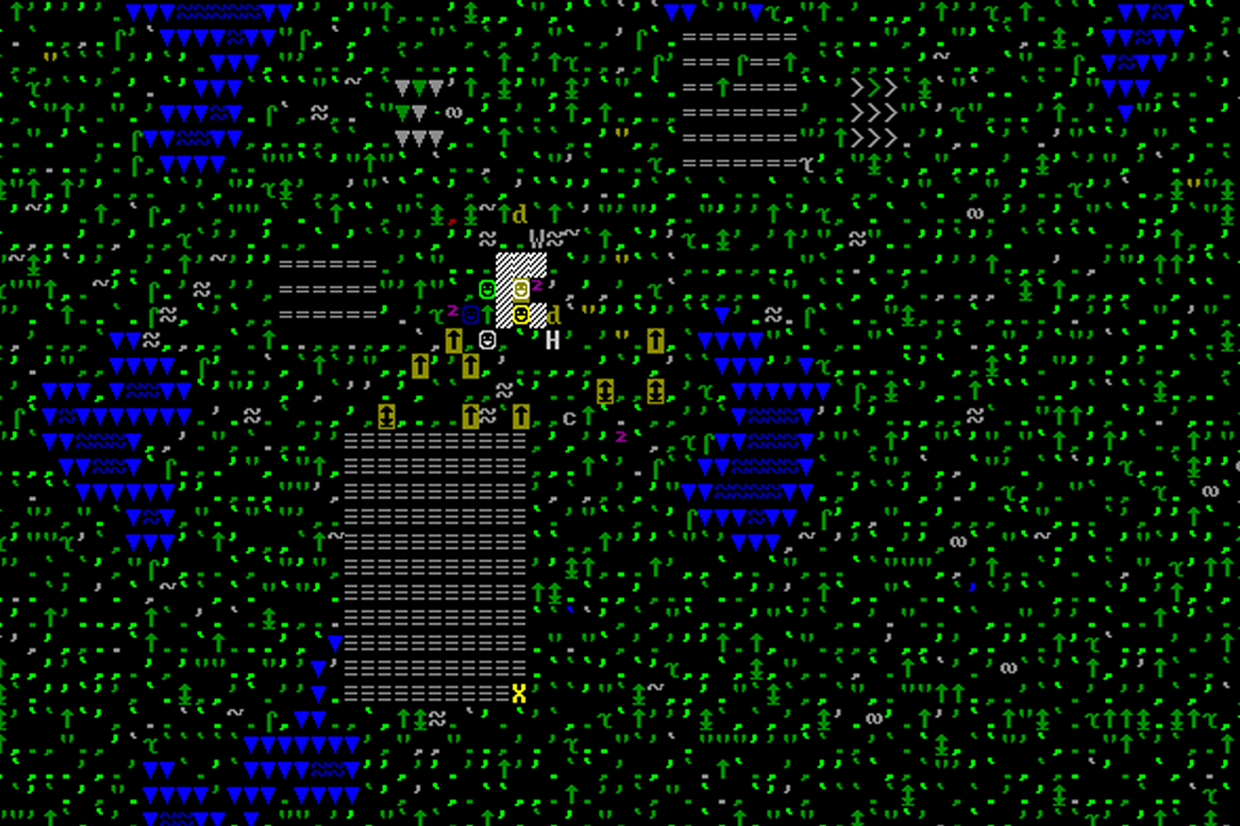
\includegraphics[width=0.45\textwidth]{df}
	\caption{Dwarf Fortress - Jeu en pixel art fait par \textit{Bay 12 Games}}
	\label{fig:df}
	\end{center}
\end{figure}

\projectTitle~est principalement inspiré du jeu \emph{Don't Move} par "stvr" (voir Figure \ref{fig:dontmove} page \pageref{fig:dontmove}). \emph{Don't Move} est un jeu indépendant qui a reçu de très bonnes critiques. Le concept du jeu est simple, si le joueur bouge, il meurt, mais en faisant cela il débloque de nouvelles fonctionnalités du jeu et de nouveaux objectifs. Le but de \projectTitle~est de pousser ce concept encore plus loin et de l'améliorer avec plus de fonctionnalités.

\begin{figure}[h]
	\begin{center}
	
\includegraphics[width=0.265\textwidth]{dontmove}
	\caption{Don't Move - jeu indépendant développé par "stvr"}
	\label{fig:dontmove}
	\end{center}
\end{figure}

\section{Description détaillée}
\projectTitle~est un jeu solo (1 joueur seulement) qui est en deux dimensions. Le jeu sera développé de manière dynamique et générique qui permettra de facilité l'ajout de contenu. Ce contenu peut être :
\begin{multicols}{2}
\begin{itemize}
	\item des armes
	\item des ennemis
	\item des nouvelles compétences
	\item de nouveaux types de points de compétences
	\item des objets de la salle
	\item des différentes disposition de la salle
	\item de nouvelles règles de jeu
\end{itemize}
\end{multicols}

\subsection{Règles}
\begin{description}
	\item Le joueur peut : sauter, se déplacer sur l'axe X, se baisser (ceci active la furtivité), attaquer avec une arme, attaquer avec de la magie et bloquer des attaques pour minimiser les dégâts.
	\item Le joueur a 100 points de vie par défaut.
	\item Les dégâts et vie des ennemis seront à définir selon le meilleur équilibre de jeu.
	\item Le joueur possède des sorts qu'il peut placer dans les touches attribuées pour les enclencher.
\end{description}

\subsection{Mécanismes}
\subsubsection{Salle}
La salle du jeu change à chaque fois que le joueur meurt. Cette salle peut avoir de nouveaux éléments, de nouvelles textures ou même de nouveaux ennemis.

\subsubsection{Points de compétences}
Le joueur peut gagner des points de compétences en tuant des ennemis ou en trouvant des pièces qui se trouve un peu partout dans la salle. Ces pièces sont défendu par des ennemis et peuvent disparaître si le joueur n'est pas discret. Il ne peut dépenser ces points après sa mort. 

\subsubsection{Compétences}
Avant de réapparaître en jeu, le joueur peut attribuer ces points sur des compétences du personnage. Par exemple, le joueur peut dépenser 2 points de compétences sur la compétence "Force" pour avoir plus de dégâts sur les coups du personnage. Voici une liste des compétences :

\begin{center}
\begin{tabularx}{\textwidth}{l X}
	\hline
	\textbf{Compétence} & \textbf{Description}\\
	\hline \hline
	Force & Apporte plus de dégâts sur les coups physiques du personnage.\\
	Agilité & Les ennemis remarquent moins le joueur et celui-ci peut se déplacer plus rapidement\\
	Vitalité & Apporte plus de points de vie au joueur\\
	Magie & Apporte plus de dégâts pour les attaques magiques du joueur\\
	\hline
\end{tabularx}
\end{center}

\subsubsection{Armes}
Les armes sont des objets pouvant être récoltés en explorant la salle. Quand le joueur trouve une arme, cette arme est mise dans l'inventaire du joueur. Le joueur pourra équiper l'arme pour faire plus de dégâts. Les armes ont des statistiques qui augmentent les dégâts physiques et/ou magiques.

\subsubsection{Sorts}
Les sorts sont des pouvoirs magiques que le joueur peut utiliser contre ses ennemis. Les dégâts magiques sont augmentés selon les points de compétences attribués à la magie. Des sorts peuvent être trouvés dans la salle sous forme de parchemin que le joueur peut ramasser, les sorts se placent dans l'inventaire et peuvent être attribués à des touches d'action (Maximum 4, touches par défaut : 1, 2, 3 ,4).

\subsection{Contrôles}
\begin{table}[htp]
\begin{center}
\begin{tabular}{|c|l|}
	\hline
	\textbf{Touche} & \textbf{Description}\\
	\hline \hline
	W & Sauter\\
	\hline
	A & Aller à gauche\\
	\hline
	D & Aller à droite\\
	\hline
	S & Se baisser (mode furtif)\\
	\hline
	Clique gauche & Attaquer (dégâts physique)\\
	\hline
	1 & Sort numéro 1\\
	\hline
	2 & Sort numéro 2\\
	\hline
	3 & Sort numéro 3\\
	\hline
	4 & Sort numéro 4\\
	\hline
	I & Afficher l'inventaire\\
	\hline
	ESC & Afficher le menu (met le jeu en pause)\\
	\hline
\end{tabular}
\end{center}
\caption{Contrôles de bases du jeu}
\end{table}
\subsection{Interface utilisateur}
L'interface utilisateur doit permettre au joueur de régler plusieurs paramètres et exécuter des actions.

\subsubsection{Options}
Les options de son, vidéo, difficulté et attribution des touches de jeu doivent être disponibles.
\subsubsection{Actions}
Il doit être possible de commencer, sauvegarder et charger une partie, puis de visualiser les scores obtenus des parties terminées.

\section{Environnement de travail}
\subsection{Inventaire hardware}
\begin{itemize}
	\item Intel Core i7 2600K @ 3.40GHz
	\item 8.00Go Dual-Channel DDR3 @ 823MHz
	\item 1024MB NVIDIA GeForce GTX 550 Ti
\end{itemize}

\subsection{Inventaire software}
\begin{itemize}
	\item Visual Studio 2013 Professional
	\item MonoGame (C\#)
\end{itemize}

\subsection{Durée et dates du projet}
Le projet se déroule sur une période de 7 semaines avec 40 heures de travail par semaine. Il y a aussi 3 jours fériés pendant le projet. Ce qui fait un total de 256 heures de travail.\\[0.3cm]
Le projet commence le lundi, 13 avril 2015 avec une reddition intermédiaire (documentation + poster) le jeudi, 30 avril 2015, puis la reddition finale le lundi, 1\textsuperscript{er} juin 2015.
\newpage
% --------------------------------------------------
\chapter{Analyse préliminaire}
\section{Analyse de l'existant}
Il n'est pas anodin de trouver des jeux similaires dans le marché du jeu-vidéo, en effet, beaucoup d'indépendants et des grandes entreprises produisent ces divertissements. Parmi les plus connus qui peuvent ressembler à \projectTitle, il existe \emph{Diablo III} et \emph{Path of Exile} qui sont des jeux récents. Ils sont similaires par rapport au type de jeu, ce sont des RPG et des Hack and Slash.

\emph{Bastion} et \emph{Transistor} sont également des jeux RPG et indépendant créer par la petite entreprise \emph{Supergiant Games}. Ces jeux sont prisés pour leur art, richesse graphique et histoire passionnante.
\section{Critique de l'existant}
\textbf{Diablo III} par \emph{Blizzard Entertainment} est actuellement le poids-lourd dans ce type de jeu, avec de hautes qualités graphiques, un contenu riche et une grande communauté active. Il est critiqué de ne pas être assez complexe et d'être trop facile à battre. 

\textbf{Path of Exile} par \emph{Grinding Gear Games} est le concurrent direct de \emph{Diablo III}, il est valorisé avec sa complexité technique dans le gameplay. Il est critiqué de ne pas être assez accessible aux joueurs lambdas et d'être trop difficile.

\textbf{Bastion} par \emph{Supergiant Games} est un jeu indépendant ayant gagné plusieurs titres pour sont originalité.
\section{Différentiation du projet}

\newpage
% --------------------------------------------------
\chapter{Analyse fonctionnelle}
\section{Personnage}
\subsection{Général}
Un personnage est contrôlé par le joueur, celui-ci peut l'équiper avec divers objets trouvé dans la salle pour augmenter ses caractéristiques. Il peut utiliser des sorts et ses armes pour vaincre ses ennemis. Le personnage possède \textbf{100} points de vie par défaut, ces points de vie augmente si le joueur décide d'améliorer sa vitalité avec des points de compétences ou des objets.

Le personnage possède 4 compétences de bases (voir section \ref{sec:competences}), il peut gagner des compétences en tuant des ennemis ou en trouvant des pièces dans la salle.

Il possède \textbf{200} points de mana qu'il peut dépenser pour utiliser des sorts. Le mana se régénéré avec le temps de \textbf{20} points de mana par seconde. 
\subsection{Inventaire}
Le personnage possède un inventaire qui sert à stocker ses objets sur soi. Les objets stocké dans l'inventaire prennent une certaine place à l'intérieur. Il n'est pas de taille infini.
\section{Compétences}
\label{sec:competences}
Les compétences sont des caractéristiques pouvant être augmenter par le personnage. Ils permettent d'augmenter ses capacités. Il existe plusieurs compétences qui sont :

\begin{description}
	\item[Force] Apporte plus de dégats sur les coups physiques
	\item[Agilité] Le personnage est plus discret et peut se déplacer plus rapidement
	\item[Vitalité] Augmente les points de vie du personnage
	\item[Magie] Augmente les dégâts magiques du personnage
\end{description}

\begin{figure}[ht]
\centering
\subfigure[Force]{%

\includegraphics[width=.20\textwidth]{strenght}
\label{fig:strenghtlogo}}
\subfigure[Agilité]{%

\includegraphics[width=.20\textwidth]{agility}
\label{fig:agilitylogo}}
\subfigure[Vitalité]{%

\includegraphics[width=.20\textwidth]{vitality}
\label{fig:vitalitylogo}}
\subfigure[Magie]{%

\includegraphics[width=.20\textwidth]{magic}
\label{fig:magiclogo}}
%
\caption{Logos des compétences}
\label{fig:competences}
\end{figure}

\section{Looting}
Le \emph{looting} est le moyen de trouver des objets. Lorsque qu'un ennemi meurt ou que l'on ouvre un coffre, par exemple, celui-ci fait tomber des objet. Cette action est appelée le \emph{looting}.
\section{Caractéristiques}
Les caractéristiques sont des propriétés qui augmente les capacités du personnages. Les compétences sont des caractéristiques mais qui peuvent être augmenter par le héro, alors que les caractéristiques peuvent seulement être augmenter par des objets.\\

\textbf{Liste des caractéristiques}
\begin{description}[labelindent=0.3cm]
    \item[Force] Le nombre de points de compétences de type \emph{Force} ajouté
    \item[Agilité] Le nombre de points de compétences de type \emph{Agilité} ajouté
    \item[Vitalité] Le nombre de points de compétences de type \emph{Vitalité} ajouté
    \item[Magie] Le nombre de points de compétences de type \emph{Magie} ajouté
    \item[Vitesse d'attaque] Le pourcentage de vitesse d'attaque ajouté au personnage
    \item[Vitesse d'attaque initial] La vitesse d'attaque initial du personnage
    \item[Dégâts] Les dégâts infligés après chaque attaque
    \item[Dégâts magiques] Les dégâts magiques infligés après chaque attaque
    \item[Armure] Déduit les dégâts reçu
    \item[Resistance magique] Déduit les dégâts magiques reçu
    \item[Régénération de vie] Régénère les points de vie
    \item[Régénération de mana] Régénère les points de mana
\end{description}
\begin{table}[ht]
\begin{center}
\begin{tabularx}{\textwidth}{| l | Y |}
  \hline                     
  Force 				& Augmente les dégâts de \textbf{1\%}\\ \hline
  Agilité 				& Diminue la distance de vue des ennemi de \textbf{0.0625\%}. Il augmente aussi la vitesse de déplacement de \textbf{0.075\%} \\ \hline
  Vitalité 				& Augmente les points de vie de \textbf{100} \\ \hline
  Magie 				& Augmente les dégâts magiques de \textbf{1\%} \\ \hline
  Vitesse d'attaque 	& Augmente la vitesse d'attaque selon la valeur en \textbf{pourcentage} \\ \hline
  Vitesse d'attaque initial	& Vitesse d'attaque initial du personnage\\ \hline
  Dégâts 				& S'ajoute au dégâts du personnage \underline{avant} d'appliquer la \emph{force} \\ \hline
  Dégâts magiques 		& S'ajoute au dégâts magiques du personnage \underline{avant} d'appliquer la \emph{magie} \\ \hline
  Armure 				& Diminue les dégâts reçu de \textbf{0.075\%} \\ \hline
  Resistance magique 	& Diminue les dégâts magiques reçu de \textbf{0.075\%} \\ \hline
  Régénération de vie 	& Augmente la régénération de points de vie selon la valeur\\ \hline
  Régénération de mana 	& Augmente la régénération de points de mana selon la valeur\\ \hline
  Vitesse de déplacement initial& Fixe la vitesse de déplacement de base du personnage\\ \hline
  Vitesse de déplacement& Augmente la vitesse de déplacement\\ \hline
\end{tabularx}
\caption{Fonctionnement des caractéristiques}
\end{center}
\end{table}
\section{Équipement}
Les équipements sont des objets que le personnage peut équiper sur lui-même pour augmenter ses points de compétences. Il existe des différents types d'objets.
\begin{itemize}
	\item Accessoires
	\item Armes
	\item Armures
\end{itemize}
%\begin{table}[H]
%\begin{center}
%\begin{tabular}{| l | c | c | c |}
%  \hline      
%  Niveau 				& 1 & 2 & 3\\ \hline \hline                 
%  Force 				& 2 & 3 & 4\\ \hline
%  Agilité 				& 5 & 6 & 4\\ \hline
%  Vitalité 			& 8 & 9 & 4\\ \hline
%  Magie 				& 8 & 9 & 4\\ \hline
%  Vitesse d'attaque 	& 8 & 9 & 4\\ \hline
%  Dégâts 				& 8 & 9 & 4\\ \hline
%  Dégâts magiques 		& 8 & 9 & 4\\ \hline
%  Armure 				& 8 & 9 & 4\\ \hline
%  Resistance magique 	& 8 & 9 & 4\\ \hline
%\end{tabular}
%\caption{Valeurs des caractéristiques}
%\end{center}
%\end{table}
\subsection{Accessoires}
\label{subsec:accessoires}
Les accessoires sont des objets spéciaux qui apporte des capacités spéciales au personnage.
\begin{multicols}{2}
\begin{itemize}
    \item Amulette
    \item Bagues
    \item Carquois
    \item Bouclier
    \item Source de pouvoir
\end{itemize}
\end{multicols}
\subsubsection{Amulette et bagues}
Ces objets apportent aléatoirement 2 à 4 des caractéristiques suivants :
\begin{table}[ht]
\begin{center}
\begin{tabular}{| l | c | c | c |}
  \hline      
  Niveau 				& 1    & 2 & 3\\ \hline \hline                 
  Force 				& 3 - 10 & 15 - 30 & 45 - 100\\ \hline
  Agilité 				& 3 - 10 & 15 - 30 & 45 - 100\\ \hline
  Vitalité 				& 3 - 10 & 15 - 30 & 45 - 100\\ \hline
  Magie 				& 3 - 10 & 15 - 30 & 45 - 100\\ \hline
  Résistance magique 	& 2 - 5  & 10 - 20 & 30 - 55\\ \hline
  Régénération de vie 	& 10 - 80  & 100 - 450 & 500 - 1000\\ \hline
  Régénération de mana 	& 1 - 5  & 6 - 13 & 14 - 20\\ \hline
\end{tabular}
\caption{Valeurs des caractéristiques d'une bague et d'une amulette}
\end{center}
\end{table}
\subsubsection{Carquois}
Le carquois apporte toujours ces caractéristiques :
\begin{multicols}{2}
\begin{itemize}
	\item Vitesse d'attaque
	\item Agilité
\end{itemize}
\end{multicols}
Il apporte aussi 0 à 3 de ces caractéristiques :
\begin{multicols}{2}
\begin{itemize}
    \item Force
    \item Vitalité
    \item Magie
    \item Régénération de vie
    \item Régénération de mana
\end{itemize}
\end{multicols}
\begin{table}[H]
\begin{center}
\begin{tabular}{| l | c | c | c |}
  \hline      
  Niveau 				& 1 & 2 & 3\\ \hline \hline                 
  Force 				& 1 - 5 & 7 - 25 & 35 - 80\\ \hline
  Agilité 				& 3 - 10 & 15 - 30 & 45 - 100\\ \hline
  Vitalité 				& 1 - 5 & 7 - 25 & 35 - 80\\ \hline
  Magie 				& 1 - 5 & 7 - 25 & 35 - 80\\ \hline
  Vitesse d'attaque 	& 1.5\% - 2.0\% & 2.5\% - 3.5\% & 4.0\% - 7.0\%\\ \hline
  Régénération de vie 	& 10 - 80  & 100 - 450 & 500 - 1000\\ \hline
  Régénération de mana 	& 1 - 5  & 6 - 13 & 14 - 20\\ \hline
\end{tabular}
\caption{Valeurs des caractéristiques du carquois}
\end{center}
\end{table}
\subsubsection{Bouclier}
Le bouclier apporte toujours ces caractéristiques :
\begin{multicols}{2}
\begin{itemize}
	\item Armure
	\item Vitalité
\end{itemize}
\end{multicols}
Il apporte aussi 0 à 3 de ces caractéristiques :
\begin{multicols}{2}
\begin{itemize}
    \item Force
    \item Agilité
    \item Magie
    \item Résistance magique
    \item Régénération de vie
    \item Régénération de mana
\end{itemize}
\end{multicols}
\begin{table}[ht]
\begin{center}
\begin{tabular}{| l | c | c | c |}
  \hline      
  Niveau 				& 1 & 2 & 3\\ \hline \hline                 
  Force 				& 1 - 5 & 7 - 25 & 35 - 80\\ \hline
  Agilité 				& 1 - 5 & 7 - 25 & 35 - 80\\ \hline
  Vitalité 				& 3 - 10 & 15 - 30 & 45 - 100\\ \hline
  Magie 				& 1 - 5 & 7 - 25 & 35 - 80\\ \hline
  Armure 				& 3 - 10 & 15 - 30 & 45 - 100\\ \hline
  Resistance magique 	& 3 - 10 & 15 - 30 & 45 - 100\\ \hline
  Régénération de vie 	& 10 - 80  & 100 - 450 & 500 - 1000\\ \hline
  Régénération de mana 	& 1 - 5  & 6 - 13 & 14 - 20\\ \hline
\end{tabular}
\caption{Valeurs des caractéristiques du bouclier}
\end{center}
\end{table}
\subsubsection{Source de pouvoir}
La source de pouvoir apporte toujours ces caractéristiques :
\begin{multicols}{2}
\begin{itemize}
	\item Magie
	\item Dégâts magiques
\end{itemize}
\end{multicols}
Elle apporte aussi 0 à 2 de ces caractéristiques :
\begin{multicols}{2}
\begin{itemize}
    \item Agilité
    \item Vitalité
    \item Vitesse d'attaque
    \item Régénération de vie
    \item Régénération de mana
\end{itemize}
\end{multicols}
\begin{table}[ht]
\begin{center}
\begin{tabular}{| l | c | c | c |}
  \hline      
  Niveau 				& 1 & 2 & 3\\ \hline \hline
  Agilité 				& 1 - 5 & 7 - 25 & 35 - 80\\ \hline
  Vitalité 				& 1 - 5 & 7 - 25 & 35 - 80\\ \hline
  Magie 				& 5 - 15 & 20 - 35 & 50 - 120\\ \hline
  Vitesse d'attaque 	& 1.5\% & 2.0\% - 3.0\% & 3.5\% - 5.0\%\\ \hline
  Dégâts magiques 		& 10 - 20 & 30 - 60 & 70 - 120\\ \hline
  Régénération de vie 	& 10 - 80  & 100 - 450 & 500 - 1000\\ \hline
  Régénération de mana 	& 1 - 5  & 6 - 13 & 14 - 20\\ \hline
\end{tabular}
\caption{Valeurs des caractéristiques de la source de pouvoir}
\end{center}
\end{table}
\subsection{Armes}
\begin{multicols}{2}
\begin{itemize}
    \item Épée
    \item Épée à deux mains
    \item Hache
    \item Hache à deux mains
    \item Baguette magique
    \item Bâton magique
    \item Arc
\end{itemize}
\end{multicols}
Les armes sont séparé en plusieurs fonctions. En bleu les armes à une main, en rouge les armes à deux mains et en vert les accessoires complémentaires aux armes (voir section \ref{subsec:accessoires}).
Le personnage peut équiper plusieurs armes en même temps selon les restrictions (voir figure \ref{fig:EquipmentRestrictions}).
\begin{figure}[ht]
	\begin{center}
	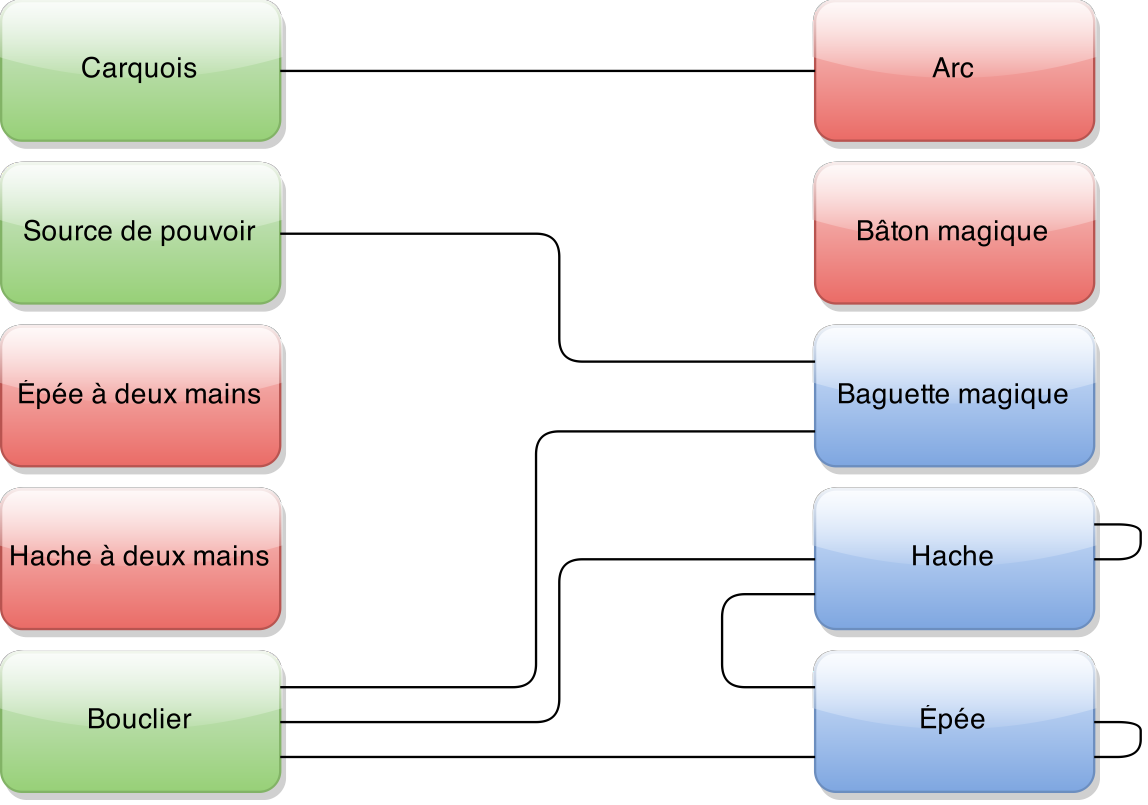
\includegraphics[width=0.8\textwidth]{EquipmentRestrictions}
	\caption{Restriction des armes}
	\label{fig:EquipmentRestrictions}
	\end{center}
\end{figure}
\subsubsection{Critères d'une arme}
Une arme est dotée de caractéristiques obligatoires qui apparaitront sur toutes les armes lootée dans le jeu:
\begin{multicols}{2}
\begin{itemize}
    \item Vitesse d'attaque initial
\end{itemize}
\end{multicols}
Elle est aussi dotée de caractéristiques optionnelles qui peuvent y figurées, certains de ces caractéristiques apparaissent obligatoirement selon le type d'objet:
\begin{multicols}{2}
\begin{itemize}
	\item Dégâts
    \item Dégâts magique
    \item Force
    \item Agilité
    \item Vitalité
    \item Magie
\end{itemize}
\end{multicols}
\subsubsection{Spécialités des type d'armes}
\begin{description}[labelindent=1cm]
    \item[Épée] Arme à une main avec la plus grande vitesse d'attaque
    \item[Épée à deux mains] Arme à deux mains avec la plus grande vitesse d'attaque
    \item[Hache] Arme à une main avec le plus de dégâts
    \item[Hache à deux mains] Arme à deux mains avec le plus de dégâts
    \item[Baguette magique] Permet d'avoir une source de pouvoir équipé en même temps.
    \item[Bâton magique] Possède de haut dégâts magiques
    \item[Arc] Haut dégâts physique à distance
\end{description}
\subsubsection{Épée}
L'épée apporte toujours ces caractéristiques :
\begin{table}[H]
\begin{center}
\begin{tabular}{| l | c | c | c |}
  \hline      
  Niveau 					& 1 & 2 & 3\\ \hline \hline                 
  Vitesse d'attaque initial	& 1.40 & 1.40 & 1.40\\ \hline
  Dégâts 					& 30 - 50 & 60 - 90 & 110 - 160\\ \hline
\end{tabular}
\caption{Valeurs des caractéristiques obligatoires de l'épée}
\end{center}
\end{table}
Elle apporte aussi 2 à 4 de ces caractéristiques :
\begin{table}[H]
\begin{center}
\begin{tabular}{| l | c | c | c |}
  \hline      
  Niveau 				& 1 & 2 & 3\\ \hline \hline                 
  Force 				& 3 - 10 & 15 - 30 & 45 - 100\\ \hline
  Agilité 				& 1 - 5 & 7 - 25 & 35 - 80\\ \hline
  Vitalité 				& 3 - 10 & 15 - 30 & 45 - 100\\ \hline
  Magie 				& 1 - 5 & 7 - 25 & 35 - 80\\ \hline
  Dégâts magiques 		& 5 - 10 & 20 - 40 & 50 - 80\\ \hline
\end{tabular}
\caption{Valeurs des caractéristiques optionnelles de l'épée}
\end{center}
\end{table}
\subsubsection{Épée à deux mains}
L'épée à deux mains apporte toujours ces caractéristiques :
\begin{table}[H]
\begin{center}
\begin{tabular}{| l | c | c | c |}
  \hline      
  Niveau 				& 1 & 2 & 3\\ \hline \hline                 
  Force 				& 3 - 10 & 15 - 30 & 45 - 100\\ \hline
  Vitesse d'attaque initial	& 1.10 & 1.10 & 1.10\\ \hline
  Dégâts 				& 65 - 110 & 120 - 190 & 230 - 360\\ \hline
\end{tabular}
\caption{Valeurs des caractéristiques obligatoires de l'épée à deux mains}
\end{center}
\end{table}
Elle apporte aussi 1 à 3 de ces caractéristiques :
\begin{table}[H]
\begin{center}
\begin{tabular}{| l | c | c | c |}
  \hline      
  Niveau 				& 1 & 2 & 3\\ \hline \hline
  Vitalité 				& 3 - 10 & 15 - 30 & 45 - 100\\ \hline
  Magie 				& 1 - 5 & 7 - 25 & 35 - 80\\ \hline
  Dégâts magiques 		& 3 - 15 & 25 - 45 & 60 - 90\\ \hline
  Régénération de vie 	& 5 - 50  & 80 - 275 & 375 - 750\\ \hline
  Régénération de mana 	& 1 - 3  & 4 - 10 & 11 - 15\\ \hline
\end{tabular}
\caption{Valeurs des caractéristiques optionnelles de l'épée à deux mains}
\end{center}
\end{table}
\subsubsection{Hache}
La hache apporte toujours ces caractéristiques :
\begin{table}[H]
\begin{center}
\begin{tabular}{| l | c | c | c |}
  \hline      
  Niveau 				& 1 & 2 & 3\\ \hline \hline                 
  Force 				& 3 - 10 & 15 - 30 & 45 - 100\\ \hline
  Vitesse d'attaque initial	& 1.30 & 1.30 & 1.30\\ \hline
  Dégâts 				& 30 - 50 & 60 - 90 & 110 - 160\\ \hline
\end{tabular}
\caption{Valeurs des caractéristiques obligatoires de la hache}
\end{center}
\end{table}
Elle apporte aussi 1 à 3 de ces caractéristiques :
\begin{table}[H]
\begin{center}
\begin{tabular}{| l | c | c | c |}
  \hline      
  Niveau 				& 1 & 2 & 3\\ \hline \hline
  Magie 				& 1 - 5 & 7 - 25 & 35 - 80\\ \hline
  Vitalité 				& 3 - 10 & 15 - 30 & 45 - 100\\ \hline
  Dégâts magiques 		& 3 - 10 & 20 - 40 & 50 - 80\\ \hline
\end{tabular}
\caption{Valeurs des caractéristiques optionnelles de la hache}
\end{center}
\end{table}
\subsubsection{Hache à deux mains}
La hache à deux mains apporte toujours ces caractéristiques :
\begin{table}[H]
\begin{center}
\begin{tabular}{| l | c | c | c |}
  \hline      
  Niveau 				& 1 & 2 & 3\\ \hline \hline                 
  Force 				& 3 - 10 & 15 - 30 & 45 - 100\\ \hline
  Vitalité 				& 3 - 10 & 15 - 30 & 45 - 100\\ \hline
  Vitesse d'attaque initial	& 1.00 & 1.00 & 1.00\\ \hline
  Dégâts 				& 65 - 110 & 120 - 190 & 230 - 360\\ \hline
\end{tabular}
\caption{Valeurs des caractéristiques obligatoires de la hache à deux mains}
\end{center}
\end{table}
Elle apporte aussi 0 à 2 de ces caractéristiques :
\begin{table}[H]
\begin{center}
\begin{tabular}{| l | c | c | c |}
  \hline      
  Niveau 				& 1 & 2 & 3\\ \hline \hline
  Magie 				& 1 - 5 & 7 - 25 & 35 - 80\\ \hline
  Dégâts magiques 		& 3 - 15 & 25 - 45 & 60 - 90\\ \hline
  Régénération de vie 	& 5 - 50  & 80 - 275 & 375 - 750\\ \hline
  Régénération de mana 	& 1 - 3  & 4 - 10 & 11 - 15\\ \hline
\end{tabular}
\caption{Valeurs des caractéristiques optionnelles de la hache à deux mains}
\end{center}
\end{table}
\subsubsection{Baguette magique}
La baguette magique apporte toujours ces caractéristiques :
\begin{table}[H]
\begin{center}
\begin{tabular}{| l | c | c | c |}
  \hline      
  Niveau 				& 1 & 2 & 3\\ \hline \hline
  Magie 				& 3 - 10 & 15 - 30 & 45 - 100\\ \hline
  Vitesse d'attaque initial	& 1.40 & 1.40 & 1.40\\ \hline
  Dégâts magiques 		& 30 - 50 & 60 - 90 & 110 - 160\\ \hline
\end{tabular}
\caption{Valeurs des caractéristiques obligatoires de la baguette magique}
\end{center}
\end{table}
Elle apporte aussi 1 à 2 de ces caractéristiques :
\begin{table}[H]
\begin{center}
\begin{tabular}{| l | c | c | c |}
  \hline      
  Niveau 				& 1 & 2 & 3\\ \hline \hline
  Agilité 				& 3 - 10 & 15 - 30 & 45 - 100\\ \hline
  Vitalité 				& 3 - 10 & 15 - 30 & 45 - 100\\ \hline
\end{tabular}
\caption{Valeurs des caractéristiques optionnelles de la baguette magique}
\end{center}
\end{table}
\subsubsection{Bâton magique}
Le bâton magique apporte toujours ces caractéristiques :
\begin{table}[H]
\begin{center}
\begin{tabular}{| l | c | c | c |}
  \hline      
  Niveau 				& 1 & 2 & 3\\ \hline \hline
  Magie 				& 3 - 10 & 15 - 30 & 45 - 100\\ \hline
  Vitesse d'attaque initial	& 1.20 & 1.20 & 1.20\\ \hline
  Dégâts magiques 		& 65 - 110 & 120 - 190 & 230 - 360\\ \hline
\end{tabular}
\caption{Valeurs des caractéristiques obligatoires du bâton magique}
\end{center}
\end{table}
Il apporte aussi 1 à 2 de ces caractéristiques :
\begin{table}[H]
\begin{center}
\begin{tabular}{| l | c | c | c |}
  \hline      
  Niveau 				& 1 & 2 & 3\\ \hline \hline
  Agilité 				& 3 - 10 & 15 - 30 & 45 - 100\\ \hline
  Vitalité 				& 3 - 10 & 15 - 30 & 45 - 100\\ \hline
  Régénération de vie 	& 5 - 50  & 80 - 275 & 375 - 750\\ \hline
  Régénération de mana 	& 1 - 3  & 4 - 10 & 11 - 15\\ \hline
\end{tabular}
\caption{Valeurs des caractéristiques optionnelles du bâton magique}
\end{center}
\end{table}
\subsubsection{Arc}
L'arc apporte toujours ces caractéristiques :
\begin{table}[H]
\begin{center}
\begin{tabular}{| l | c | c | c |}
  \hline      
  Niveau 				& 1 & 2 & 3\\ \hline \hline
  Agilité 				& 3 - 10 & 15 - 30 & 45 - 100\\ \hline
  Vitesse d'attaque initial	& 1.30 & 1.30 & 1.30\\ \hline
  Dégâts 				& 30 - 50 & 60 - 90 & 110 - 160\\ \hline
\end{tabular}
\caption{Valeurs des caractéristiques obligatoires de l'arc}
\end{center}
\end{table}
Il apporte aussi 1 à 3 de ces caractéristiques :
\begin{table}[H]
\begin{center}
\begin{tabular}{| l | c | c | c |}
  \hline      
  Niveau 				& 1 & 2 & 3\\ \hline \hline                 
  Force 				& 3 - 10 & 15 - 30 & 45 - 100\\ \hline
  Vitalité 				& 3 - 10 & 15 - 30 & 45 - 100\\ \hline
  Magie 				& 1 - 5 & 7 - 25 & 35 - 80\\ \hline
  Dégâts magiques 		& 3 - 10 & 20 - 40 & 50 - 80\\ \hline
\end{tabular}
\caption{Valeurs des caractéristiques optionnelles de l'arc}
\end{center}
\end{table}
\subsection{Armures}
\begin{multicols}{2}
\begin{itemize}
    \item Tête
    \item Épaules
    \item Corps
    \item Mains
    \item Jambes
    \item Pieds
\end{itemize}
\end{multicols}
\subsubsection{Tête}
Une armure pour la tête apporte obligatoirement ces caractéristiques :
\begin{table}[H]
\begin{center}
\begin{tabular}{| l | c | c | c |}
  \hline      
  Niveau 				& 1 & 2 & 3\\ \hline \hline
  Vitalité 				& 3 - 10 & 15 - 30 & 45 - 100\\ \hline
  Armure 				& 3 - 10 & 15 - 30 & 45 - 100\\ \hline
\end{tabular}
\caption{Valeurs des caractéristiques obligatoire de l'armure pour la tête}
\end{center}
\end{table}
Elle apporte aussi 0 à 2 de ces caractéristiques :
\begin{table}[H]
\begin{center}
\begin{tabular}{| l | c | c | c |}
  \hline      
  Niveau 				& 1 & 2 & 3\\ \hline \hline                 
  Force 				& 3 - 10 & 15 - 30 & 45 - 100\\ \hline
  Agilité 				& 3 - 10 & 15 - 30 & 45 - 100\\ \hline
  Magie 				& 3 - 10 & 15 - 30 & 45 - 100\\ \hline
  Resistance magique 	& 3 - 10 & 15 - 30 & 45 - 100\\ \hline
  Régénération de vie 	& 5 - 50  & 80 - 275 & 375 - 750\\ \hline
  Régénération de mana 	& 1 - 3  & 4 - 10 & 11 - 15\\ \hline
\end{tabular}
\caption{Valeurs des caractéristiques optionnelles de l'armure pour la tête}
\end{center}
\end{table}
\subsubsection{Épaules}
Une armure pour les épaules apporte obligatoirement ces caractéristiques :
\begin{table}[H]
\begin{center}
\begin{tabular}{| l | c | c | c |}
  \hline      
  Niveau 				& 1 & 2 & 3\\ \hline \hline
  Armure 				& 3 - 10 & 15 - 30 & 45 - 100\\ \hline
\end{tabular}
\caption{Valeurs des caractéristiques obligatoire de l'armure pour les épaules}
\end{center}
\end{table}
Elle apporte aussi 1 à 3 de ces caractéristiques :
\begin{table}[H]
\begin{center}
\begin{tabular}{| l | c | c | c |}
  \hline      
  Niveau 				& 1 & 2 & 3\\ \hline \hline                 
  Force 				& 3 - 10 & 15 - 30 & 45 - 100\\ \hline
  Agilité 				& 3 - 10 & 15 - 30 & 45 - 100\\ \hline
  Vitalité 				& 3 - 10 & 15 - 30 & 45 - 100\\ \hline
  Magie 				& 3 - 10 & 15 - 30 & 45 - 100\\ \hline
  Resistance magique 	& 3 - 10 & 15 - 30 & 45 - 100\\ \hline
\end{tabular}
\caption{Valeurs des caractéristiques optionnelles de l'armure pour les épaules}
\end{center}
\end{table}
\subsubsection{Corps}
Une armure pour le corps apporte obligatoirement ces caractéristiques :
\begin{table}[H]
\begin{center}
\begin{tabular}{| l | c | c | c |}
  \hline      
  Niveau 				& 1 & 2 & 3\\ \hline \hline
  Armure 				& 3 - 10 & 15 - 30 & 45 - 100\\ \hline
\end{tabular}
\caption{Valeurs des caractéristiques obligatoire de l'armure pour le corps}
\end{center}
\end{table}
Elle apporte aussi 1 à 3 de ces caractéristiques :
\begin{table}[H]
\begin{center}
\begin{tabular}{| l | c | c | c |}
  \hline      
  Niveau 				& 1 & 2 & 3\\ \hline \hline                 
  Force 				& 3 - 10 & 15 - 30 & 45 - 100\\ \hline
  Agilité 				& 3 - 10 & 15 - 30 & 45 - 100\\ \hline
  Vitalité 				& 3 - 10 & 15 - 30 & 45 - 100\\ \hline
  Magie 				& 3 - 10 & 15 - 30 & 45 - 100\\ \hline
  Resistance magique 	& 3 - 10 & 15 - 30 & 45 - 100\\ \hline
  Régénération de vie 	& 5 - 50  & 80 - 275 & 375 - 750\\ \hline
  Régénération de mana 	& 1 - 3  & 4 - 10 & 11 - 15\\ \hline
\end{tabular}
\caption{Valeurs des caractéristiques optionnelles de l'armure pour le corps}
\end{center}
\end{table}
\subsubsection{Mains}
Une armure pour les mains apporte obligatoirement ces caractéristiques :
\begin{table}[H]
\begin{center}
\begin{tabular}{| l | c | c | c |}
  \hline      
  Niveau 				& 1 & 2 & 3\\ \hline \hline
  Agilité 				& 3 - 10 & 15 - 30 & 45 - 100\\ \hline
  Armure 				& 3 - 10 & 15 - 30 & 45 - 100\\ \hline
\end{tabular}
\caption{Valeurs des caractéristiques obligatoire de l'armure pour les mains}
\end{center}
\end{table}
Elle apporte aussi 0 à 2 de ces caractéristiques :
\begin{table}[H]
\begin{center}
\begin{tabular}{| l | c | c | c |}
  \hline      
  Niveau 				& 1 & 2 & 3\\ \hline \hline                 
  Force 				& 3 - 10 & 15 - 30 & 45 - 100\\ \hline
  Vitalité 				& 3 - 10 & 15 - 30 & 45 - 100\\ \hline
  Magie 				& 3 - 10 & 15 - 30 & 45 - 100\\ \hline
  Resistance magique 	& 3 - 10 & 15 - 30 & 45 - 100\\ \hline
\end{tabular}
\caption{Valeurs des caractéristiques optionnelles de l'armure pour les mains}
\end{center}
\end{table}
\subsubsection{Jambes}
Une armure pour les jambes apporte obligatoirement ces caractéristiques :
\begin{table}[H]
\begin{center}
\begin{tabular}{| l | c | c | c |}
  \hline      
  Niveau 				& 1 & 2 & 3\\ \hline \hline
  Armure 				& 3 - 10 & 15 - 30 & 45 - 100\\ \hline
\end{tabular}
\caption{Valeurs des caractéristiques obligatoire de l'armure pour les jambes}
\end{center}
\end{table}
Elle apporte aussi 1 à 3 de ces caractéristiques :
\begin{table}[H]
\begin{center}
\begin{tabular}{| l | c | c | c |}
  \hline      
  Niveau 				& 1 & 2 & 3\\ \hline \hline                 
  Force 				& 3 - 10 & 15 - 30 & 45 - 100\\ \hline
  Agilité 				& 3 - 10 & 15 - 30 & 45 - 100\\ \hline
  Vitalité 				& 3 - 10 & 15 - 30 & 45 - 100\\ \hline
  Magie 				& 3 - 10 & 15 - 30 & 45 - 100\\ \hline
  Resistance magique 	& 3 - 10 & 15 - 30 & 45 - 100\\ \hline
\end{tabular}
\caption{Valeurs des caractéristiques optionnelles de l'armure pour les jambes}
\end{center}
\end{table}
\subsubsection{Pieds}
Une armure pour les pieds apporte obligatoirement ces caractéristiques :
\begin{table}[H]
\begin{center}
\begin{tabular}{| l | c | c | c |}
  \hline      
  Niveau 				& 1 & 2 & 3\\ \hline \hline
  Agilité 				& 3 - 10 & 15 - 30 & 45 - 100\\ \hline
  Vitesse de déplacement initial& 6\% - 12\% & 6\% - 12\% & 6\% - 12\%\\ \hline
  Armure 				& 3 - 10 & 15 - 30 & 45 - 100\\ \hline
\end{tabular}
\caption{Valeurs des caractéristiques obligatoire de l'armure pour les pieds}
\end{center}
\end{table}
Elle apporte aussi 0 à 2 de ces caractéristiques :
\begin{table}[H]
\begin{center}
\begin{tabular}{| l | c | c | c |}
  \hline      
  Niveau 				& 1 & 2 & 3\\ \hline \hline                 
  Force 				& 3 - 10 & 15 - 30 & 45 - 100\\ \hline
  Vitalité 				& 3 - 10 & 15 - 30 & 45 - 100\\ \hline
  Magie 				& 3 - 10 & 15 - 30 & 45 - 100\\ \hline
  Resistance magique 	& 3 - 10 & 15 - 30 & 45 - 100\\ \hline
\end{tabular}
\caption{Valeurs des caractéristiques optionnelles de l'armure pour les pieds}
\end{center}
\end{table}
\section{Sorts}
\subsection{Sort -- Bleed}
\emph{Bleed} ou saigné en français, est un sort qui inflige des dégâts continue à un ou plusieurs ennemis. Il inflige \textbf{200\%} de dégâts par secondes pendant \textbf{5} secondes dans un rayon de \textbf{10} mètres.

Le sort coûte \textbf{50} mana.\\

Disponible pour les armes suivants :
\begin{multicols}{2}
\begin{itemize}
    \item Épée à une main
    \item Hache à une main
    \item Épée à deux mains
    \item Hache à deux mains
\end{itemize}
\end{multicols}
\subsection{Sort -- Cripple}
\emph{Cripple} ou estropier en français, est un sort qui ralenti la vitesse de déplacement de l'ennemi de \textbf{80\%} et aussi sa vitesse d'attaque de \textbf{80\%} pendant \textbf{5} secondes. Le sort inflige aussi \textbf{140\%} de dégâts.

Le sort coûte \textbf{50} mana.\\

Disponible pour les armes suivants :
\begin{multicols}{2}
\begin{itemize}
    \item Épée à une main
    \item Hache à une main
\end{itemize}
\end{multicols}
\subsection{Sort -- Rapid Attack}
\emph{Rapid Attack} ou attaque rapide en français, est un sort qui augmente la vitesse d'attaque du personnage de \textbf{50\%} pendant \textbf{5} secondes.

Le sort coûte \textbf{50} mana.\\

Disponible pour les armes suivants :
\begin{multicols}{2}
\begin{itemize}
    \item Épée à une main
    \item Hache à une main
    \item Arc
\end{itemize}
\end{multicols}
\subsection{Sort -- Smash}
\emph{Smash} ou écraser en français, est un sort qui inflige \textbf{300\%} de dégâts dans un rayon de \textbf{10} mètres.

Le sort coûte \textbf{50} mana.\\

Disponible pour les armes suivants :
\begin{multicols}{2}
\begin{itemize}
    \item Épée à deux mains
    \item Hache à deux mains
\end{itemize}
\end{multicols}
\subsection{Sort -- Knock-out \& Freeze}
\emph{Knock-out} ou assommer en français, est un sort qui assomme les ennemis pendant \textbf{3} secondes et inflige \textbf{140\%} de dégâts dans un rayon de \textbf{6} mètres.

Le sort coûte \textbf{50} mana.\\

Disponible pour les armes suivants :
\begin{multicols}{2}
\begin{itemize}
    \item Épée à deux mains
    \item Hache à deux mains
\end{itemize}
\end{multicols}
\subsection{Sort -- Freeze}
\emph{Freeze} ou geler en français, est un sort qui gèle les ennemis pendant \textbf{3} secondes et inflige \textbf{140\%} de dégâts magiques dans un rayon de \textbf{6} mètres.

Le sort coûte \textbf{50} mana.\\

Disponible pour les armes suivants :
\begin{multicols}{2}
\begin{itemize}
    \item Bâton magique
    \item Baguette magique
\end{itemize}
\end{multicols}
\subsection{Sort -- Armor-up}
\emph{Armor-up} ou augmenter l'armure en français, est un sort qui augmente l'armure et la résistance magique du personnage de \textbf{100\%} pendant \textbf{5} secondes.

Le sort coûte \textbf{50} mana.\\

Disponible pour les armes suivants :
\begin{multicols}{2}
\begin{itemize}
    \item Bâton magique
    \item Baguette magique
\end{itemize}
\end{multicols}
\subsection{Sort -- Fast}
\emph{Fast} ou rapide en français, est un sort qui augmente la vitesse de déplacement du personnage de \textbf{100\%} pendant \textbf{5} secondes.

Le sort coûte \textbf{50} mana.\\

Disponible pour les armes suivants :
\begin{multicols}{2}
\begin{itemize}
    \item Épée à une main
    \item Hache à une main
    \item Arc
\end{itemize}
\end{multicols}
\subsection{Sort -- Zone-Damage}
\emph{Zone-Damage} ou dégâts de zone en français, est un sort qui inflige \textbf{600\%} de dégâts dans un rayon de \textbf{15} mètres.

Il inflige \textbf{600\%} de dégâts magique si le personnage est équipé d'un bâton magique ou d'une baguette magique.

Le sort coûte \textbf{50} mana.\\

Disponible pour les armes suivants :
\begin{multicols}{2}
\begin{itemize}
    \item Bâton magique
    \item Baguette magique
    \item Arc
\end{itemize}
\end{multicols}
\section{Ennemis}
Il y a 3 ennemis de bases de différentes tailles : petite, moyenne et grande.
\subsection{Boss final -- Hel}
\section{Monde}
Le monde du jeu est basé sur un concept simple. Le personnage commence dans un village (base principale) où il peut trouver un coffre et un portail pour se téléporter.
Le portail mène vers un niveau (le terrain de combat) généré d'où il ne peut plus revenir dans le village sans mourir. Ce niveau est composé de 3 zone de difficultés, chacun plus difficile que l'autre.
\subsection{Village}
En cours d'un jeu, le joueur apparait dans un vilage où il y a a disposition, un coffre de stockage et des teleporteurs pour aller dans les différentes cartes.
\newpage
% --------------------------------------------------
\chapter{Analyse organique}
\section{Monogame}
Monogame fournit des fonctionnalités indispensable pour le développement d'un jeu. Il offre la boucle de jeu de base qui permet de mettre à jour tous les éléments du programme (voir figure \ref{fig:loopmg}) ainsi que beaucoup de classe utiles pour le développement de jeu.
\begin{figure}[H]
	\begin{center}
	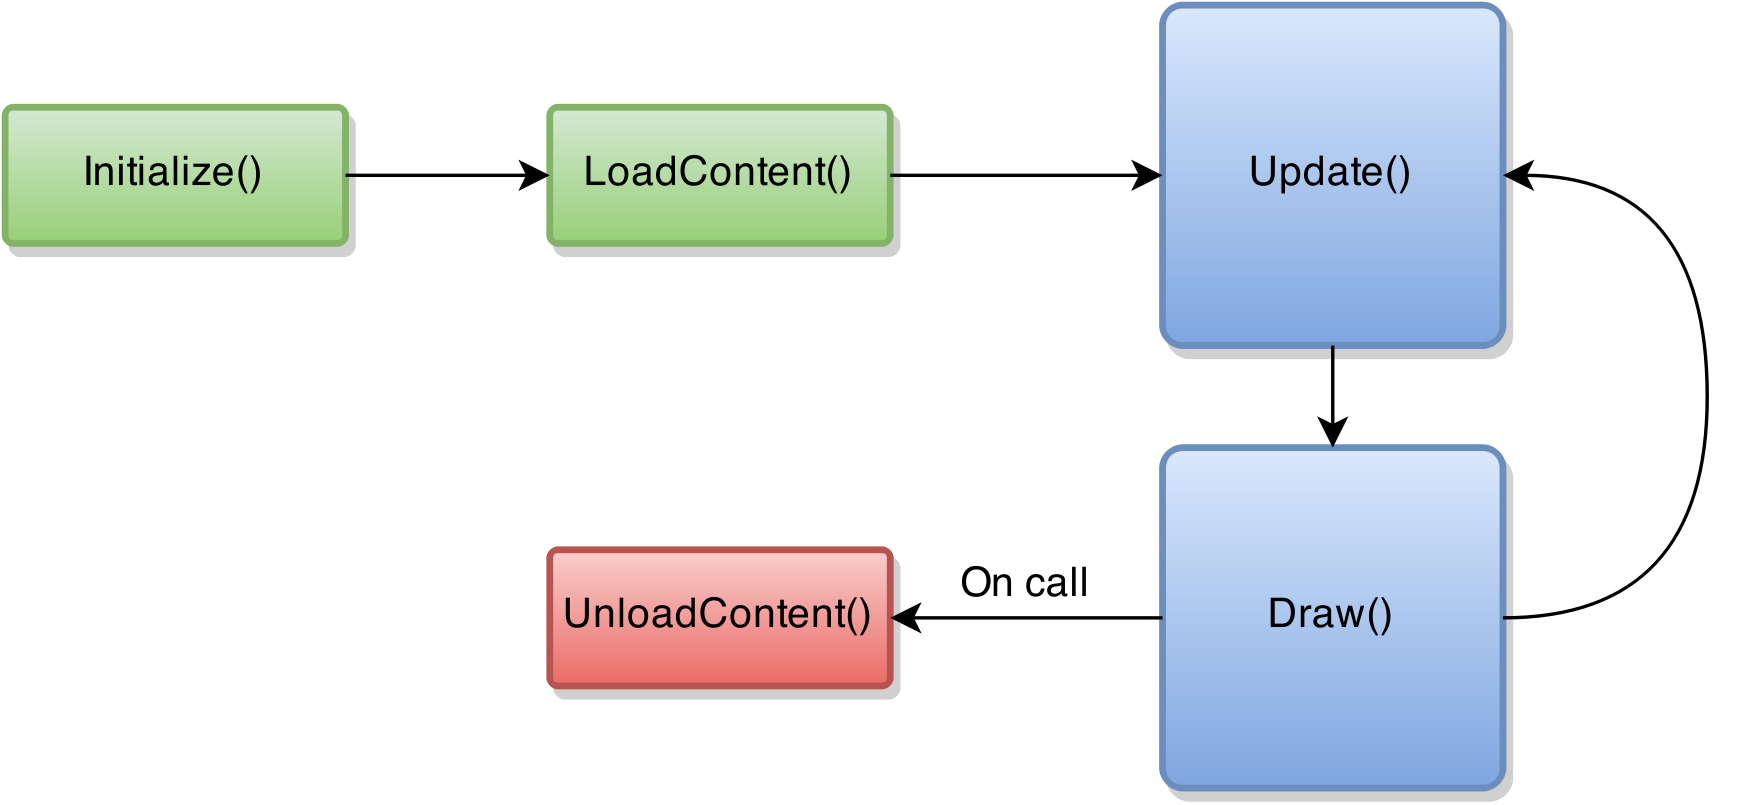
\includegraphics[width=0.8\textwidth]{loopmg}
	\caption{Boucle du framework MonoGame}
	\label{fig:loopmg}
	\end{center}
\end{figure}
\subsection{Les boucles de jeu}
\subsubsection{La boucle \textit{LoadContent}}
La boucle \textit{LoadContent} sert à initialiser du contenu. Cette méthode peut se retrouver dans des classes pour initialiser le contenu de la classe comme les textures par exemple. La méthode est appelée une fois lors de l'initialisation.
\subsubsection{La boucle \textit{UnloadContent}}
La boucle \textit{UnloadContent} sert à retirer les variables comme les textures pour être sûr de leurs déchargement. La méthode est appelée seulement implicitement ou lors de la fermeture du programme.
\subsubsection{La boucle \textit{Update}}
La boucle \textit{Update} sert à mettre à jour tous les contenu non-graphique du jeu. Cette méthode peut se retrouver dans des classes qui nécessite d'étre mis-à-jour régulièrement quand il est possible. Elle est appelée constamment par Monogame.
\subsubsection{La boucle \textit{Draw}}
La boucle \textit{Draw} dessine le contenu sur l'écran du jeu. Cette méthode peut se retrouver dans des classes pour dessiner son contenu. Il est appelé constamment quand il est possible, car la boucle Update possède la priorité et si celui-ci est chargée, Monogame ignorera la méthode \textit{Draw}.
\subsection{Les fonctionnalités utiles pour le projet}
Monogame offre une gamme de fonctionnalités et de classes. 

\section{La structure du projet}
\subsection{Architecture du jeu}
\begin{figure}[H]
	\begin{center}
	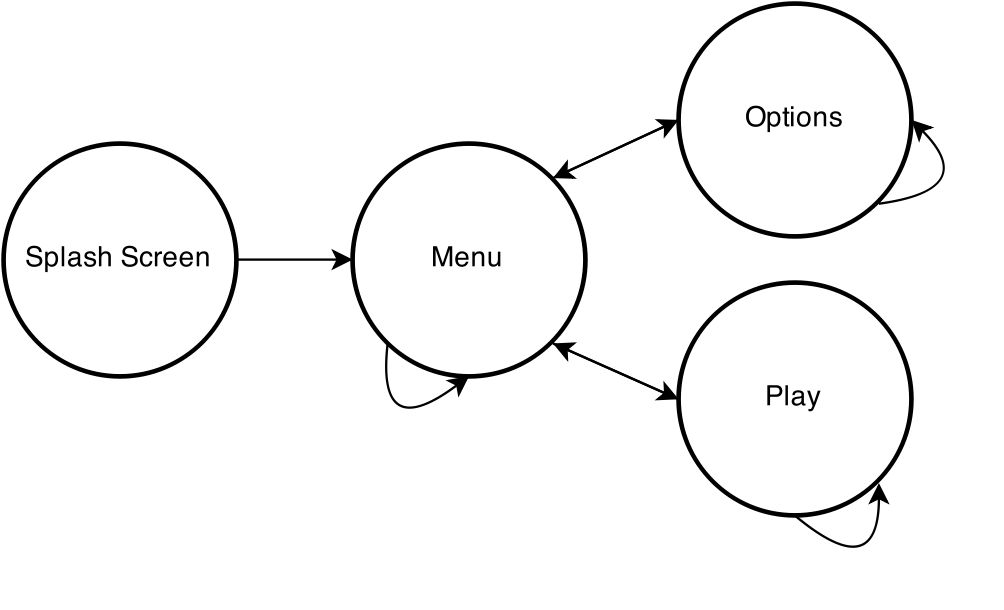
\includegraphics[width=0.8\textwidth]{StatesOfProgram}
	\caption{Différents états du programme}
	\label{fig:StatesOfProgram}
	\end{center}
\end{figure}
\begin{figure}[H]
	\begin{center}
	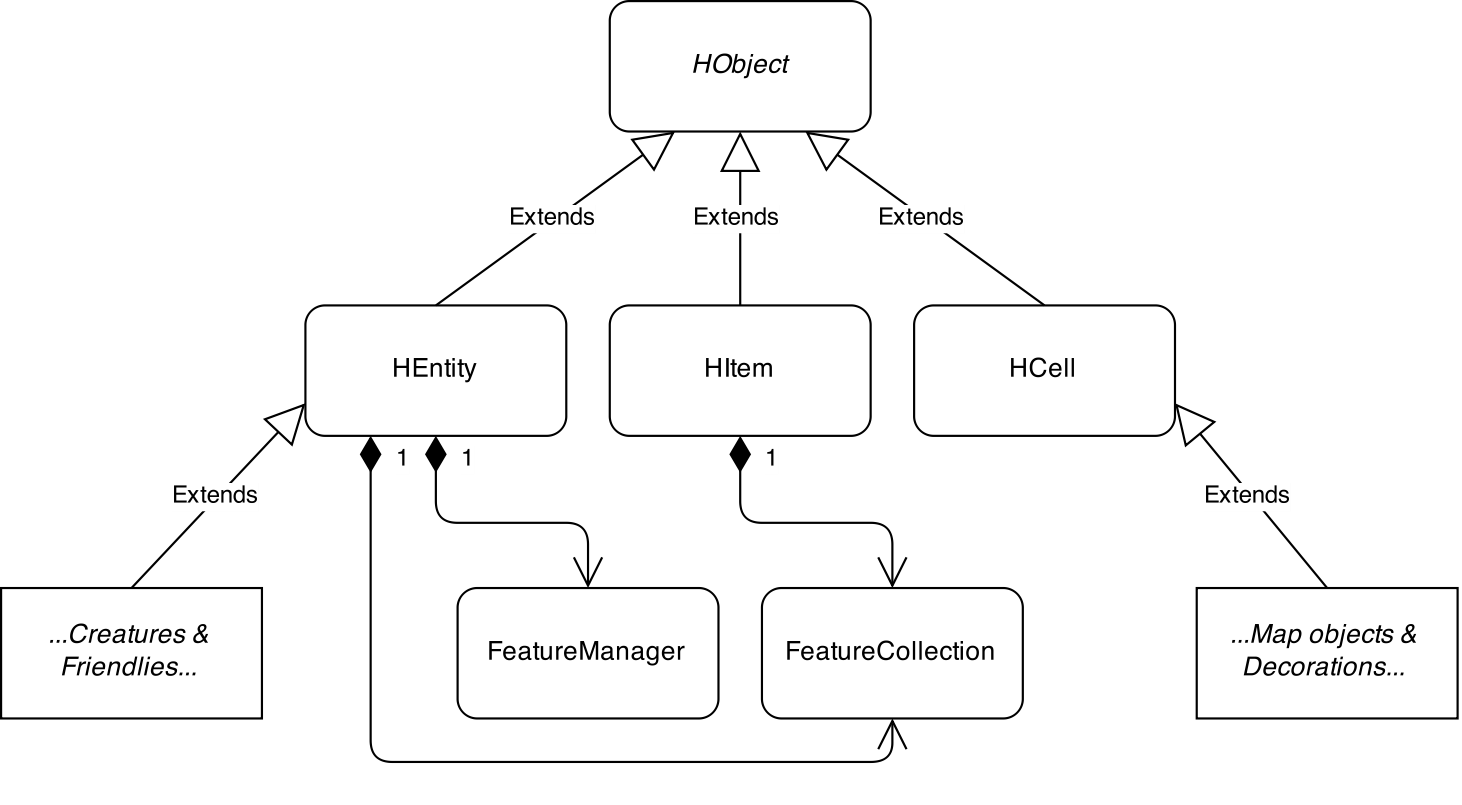
\includegraphics[width=1\textwidth]{WorldObjects}
	\caption{Schémas de hiérarchisation des objets du monde}
	\label{fig:WorldObjects}
	\end{center}
\end{figure}
\subsection{Classe de jeu de base}
\label{subsec:classdebase}
Tout les éléments du jeu hérite de la classe HObject, ce qui permet une grande simplification pour le développement (Voir figure  \ref{fig:HObject}). Cette classe abstraite présente :\\(\textit{\textbf{f}} signifie que c'est une méthode de la classe et \textit{\textbf{p}} signifie que c'est une propriété de la classe.)
\begin{description}[labelindent=0.5cm]
	\item[\textit{p} IsWalkable] permet de savoir si l'élément peut être superposé avec un autre.
	\item[\textit{p} Position] position précise relative à la carte.
	\item[\textit{f} LoadContent] permet de charger du contenu.
	\item[\textit{f} UnloadContent] permet de décharger du contenu.
	\item[\textit{f} Update] permet de mettre à jour l'objet.
	\item[\textit{f} Draw] permet de dessiner l'objet sur l'écran.
\end{description}
\begin{figure}[h]
	\begin{center}
	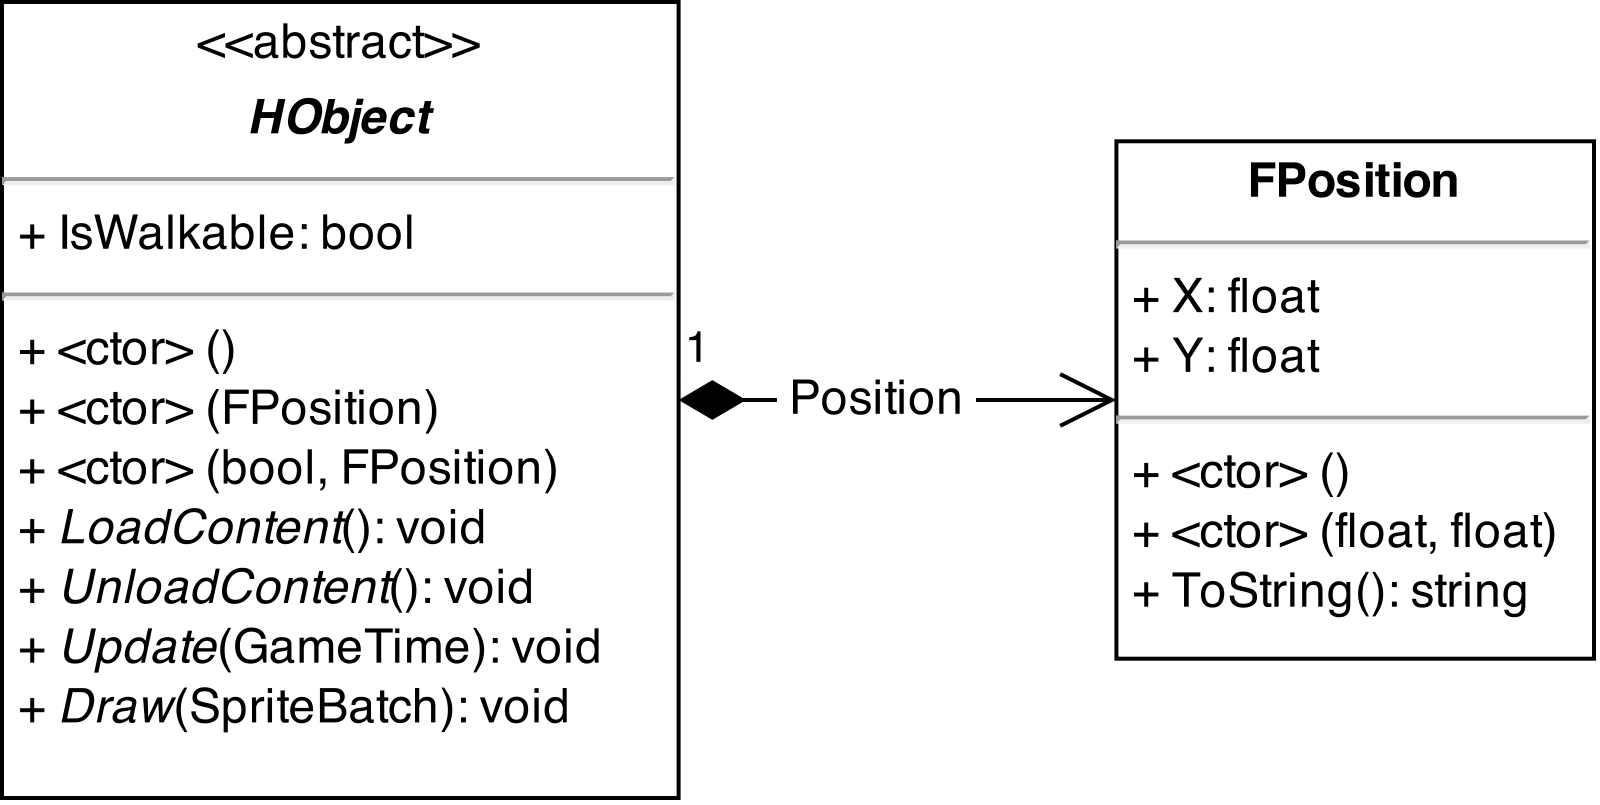
\includegraphics[width=0.8\textwidth]{HObject}
	\caption{Diagramme de classe de HObject}
	\label{fig:HObject}
	\end{center}
\end{figure}
\newpage
\section{Gestion de la carte}
La carte est constituée d'un tableau à deux dimensions de classe \emph{HCell}. Il possède une hauteur et une largeur ainsi qu'une liste de tous les objets et ennemis présent. Des fonctions de bases pour \emph{get/set} les cellules sont nécessaires :
\begin{itemize}
	\item Prendre une cellule \textbf{désignée}
	\item Prendre les cellules \textbf{voisines} d'une cellule
	\item Prendre les cellules \textbf{voisines non-accessible} d'une cellule
	\item Prendre le \textbf{nombre} de cellules voisines non-accessible d'une cellule
	\item Prendre la cellule se trouvant \textbf{dessous} d'une cellule
	\item Prendre la cellule se trouvant \textbf{dessus} d'une cellule
	\item Prendre la cellule se trouvant \textbf{à gauche} d'une cellule
	\item Prendre la cellule se trouvant \textbf{à droite} d'une cellule
	\item Prendre une cellule \textbf{aléatoire} et qui est \textbf{accessible}
\end{itemize}
\subsection{Cellules}
Les cellules hérite de \textit{HObject}\footnote{Voir section \ref{subsec:classdebase} pour les objets de bases} et ils possèdent des limites et un type. Les limites est de type \textit{FRectangle}\footnote{Voir section \ref{subsec:intersections} pour la classe float rectangle} ce qui permet de détecter les intersections avec les autres objets. Le type de la cellule est un string qui permet de l'identifier, ce string peut être lié à une texture du \textit{TextureManager}\footnote{Voir section \ref{subsec:texturemanager} pour la gestion de texture}.
\subsection{Génération de la carte}
La génération est faite grâce a un algorithme d'automate cellulaire modifié pour créer des apparences de cavernes. Chaque cellule, selon son état et ses voisins peut changer. Dans ce cas, ce sont des cellules carrés placées dans un tableau à deux dimensions. Une cellule possède donc au maximum 8 voisins en comptant les diagonales. Il est bien sûr possible d'augmenter l'étendu des voisins pour compter plus de variables et augmenter la taille des salles de la caverne.

Afin de créer un effet aléatoire, il est nécessaire d'initialiser le tableau avec environ 40\% de cellules pleines et avec des bords plein, afin d'éviter que le joueur ne parte de la carte. L'algorithme peut ensuite être appliquer au tableau. Il est nécessaire de l'appliquer plusieurs fois pour augmenter les aspects \emph{naturels} d'une caverne (voir figure \ref{fig:mapgeneration}).
\begin{figure}[H]
	\begin{center}
	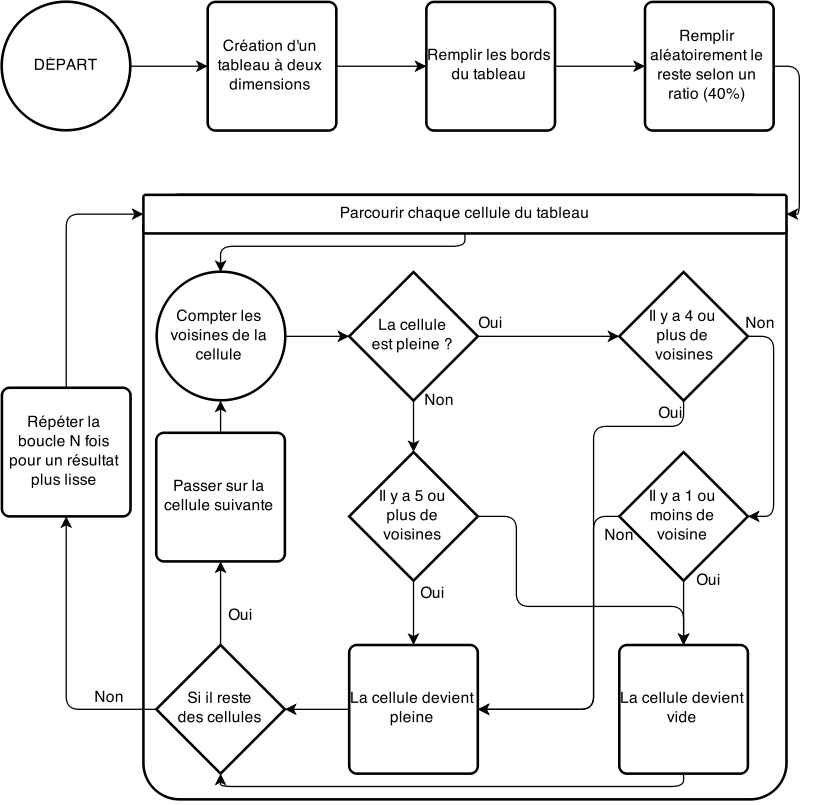
\includegraphics[width=1\textwidth]{mapgeneration}
	\caption{Diagramme de flux de la génération de carte (cavernes)}
	\label{fig:mapgeneration}
	\end{center}
\end{figure}
\section{Éléments du jeu}
\subsection{Caractéristiques}
\label{subsec:caracteristiques}
Les caractéristique font l'essence même du jeu. Il faut qu'il soit placé dans tous les entités du jeu, parce que ceux-ci se repose dessus pour tous leurs actions. Les objets ou "items" sont des choses que les entités peuvent porter pour augmenter leurs caractéristiques global (Voir figure \ref{fig:FeatureGlobalWork}).
Pour gérer tous les calculs entre les caractéristique, un manager de caractéristiques doit être placé sur l'entité. Le manager analysera tous les éléments possédant des caractéristique et fera une somme global pour fixer les caractéristiques final de l'entité.
\begin{figure}[H]
	\begin{center}
	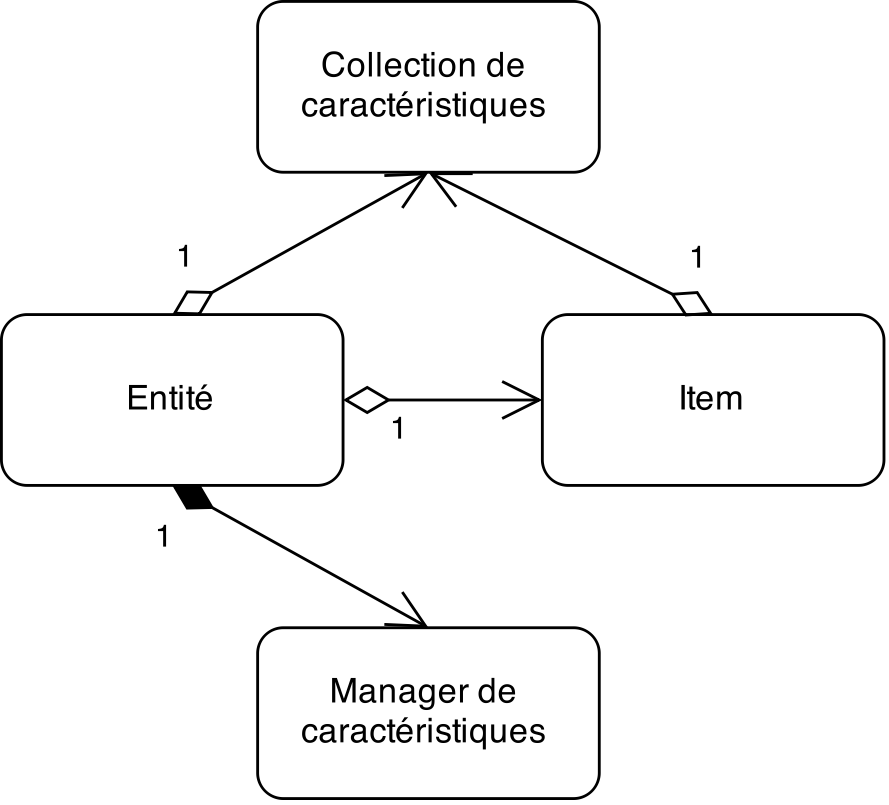
\includegraphics[width=0.5\textwidth]{FeatureGlobalWork}
	\caption{Schémas simple de fonctionnement des caractéristiques}
	\label{fig:FeatureGlobalWork}
	\end{center}
\end{figure}
\begin{figure}[H]
	\begin{center}
	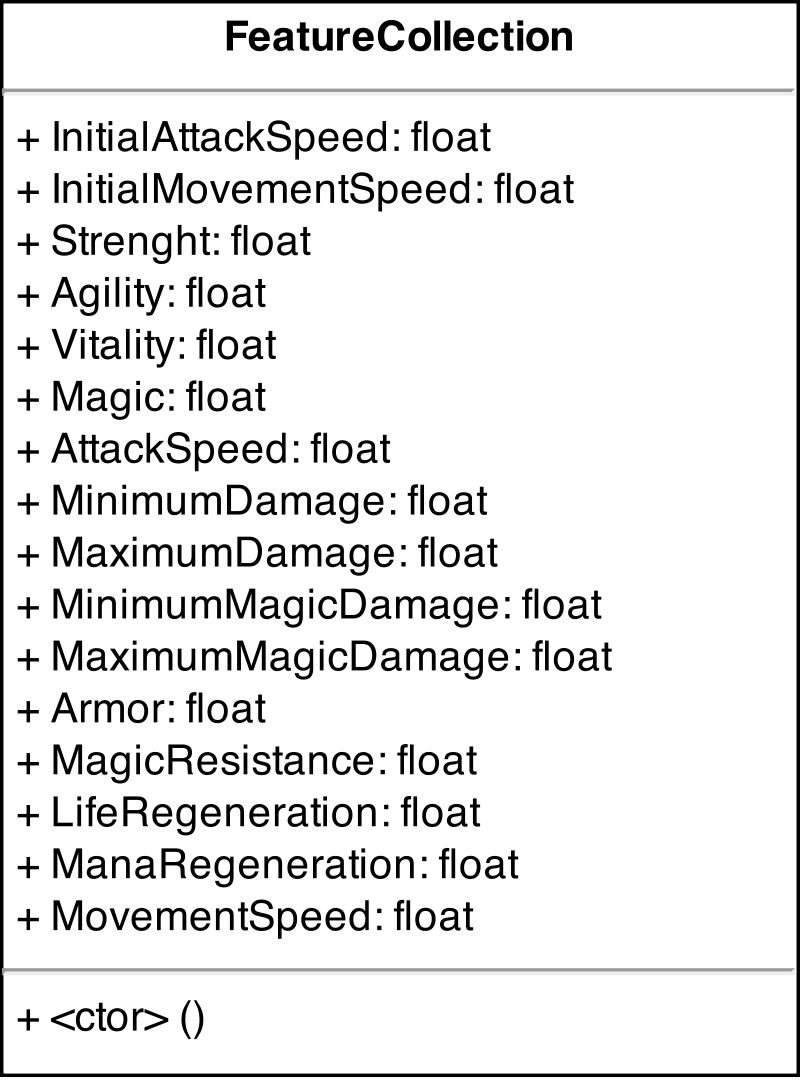
\includegraphics[width=0.35\textwidth]{FeatureCollection}
	\caption{Diagramme de classe de la collection de caractéristiques}
	\label{fig:FeatureCollection}
	\end{center}
\end{figure}
Le \textit{FeatureCollection} est la classe qui permet de stocker ces caractéristiques. Elle ne fait rien de spécial sauf stocker ses valeurs. C'est pourquoi trois propriétés de caractéristiques existe sur une entité (voir listing \ref{lst:maxforceentity}) :
\begin{description}[labelindent=0.5cm]
	\item[InitialValue] Les caractéristiques initial de l'entité
	\item[MaximizedFeatures] Les caractéristiques maximum en tenant compte des sorts et des objets qu'il porte.
	\item[ActualFeatures] Les caractéristiques en tenant compte des sorts et des objets qu'il porte et aussi de dégâts et effets néfaste de l'entité.
\end{description}
Voir figure \ref{fig:FeatureCollection} pour le diagramme de classe d'une collection de caractéristiques.
\begin{lstlisting}[caption=Exemple de calcul de la force maximal d'une entité, label=lst:maxforceentity]
/// <summary>
/// Calculates the total strenght within the items, spells and initial values
/// </summary>
/// <returns>Total strenght</returns>
public float GetTotalStrenght() {
	// Gets the initial strenght of the entity
	float str = this.InitialFeatures.Strenght;
	// For each currently active spell, we add the strenght of it
	for (int i = 0; i < this.ActiveSpells.Count; i++)
	{
		str += this.ActiveSpells[i].Features.Strenght;
	}
	// For each worn item of the entity, we add the strenght of it
	for (int i = 0; i < this.ActiveItems.Count; i++)
	{
		str += this.ActiveItems[i].Features.Strenght;
	}
	return str; // return the total
	
}
\end{lstlisting}
\subsection{La classe entité}
La classe entité (\textit{HEntity}, voir figure \ref{fig:HEntity}) est une classe abstraite qui forme la base de tous les entités "intelligent" du jeu. C'est-à-dire des unités qui possèdent des caractéristiques pour interagir avec le joueur.
\begin{figure}[h]
	\begin{center}
	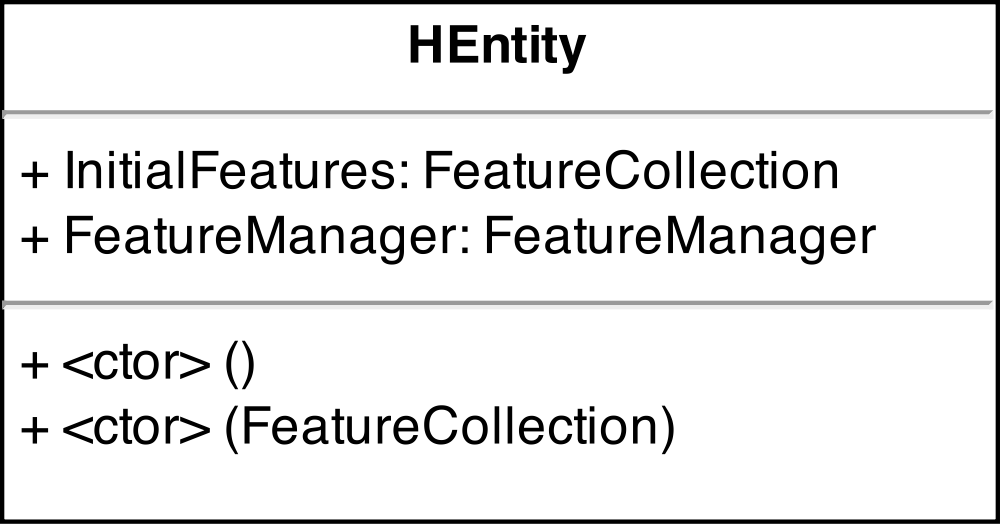
\includegraphics[width=.6\textwidth]{HEntity}
	\caption{Diagramme de classe d'une entité du jeu}
	\label{fig:HEntity}
	\end{center}
\end{figure}
Pour une explication de InitialFeatures, ActualFeatures et MaximizedFeatures, voir la section \ref{subsec:caracteristiques} sur les caractéristiques.

\subsubsection{Les états}
Une entité doit également posséder un état pour savoir ce qu'il es en train de faire. Ses états sont les suivants : 
\begin{description}[labelindent=0.5cm]
	\item[S0 Idle] Il ne fait rien
	\item[S1 Running] Il est en déplacement
	\item[S2 MeleeAttacking] Il exécute une attaque au corps-à-corps
	\item[S3 RangeAttacking] Il exécute une attaque à distance
	\item[S4 SpellCasting] Il exécute un sort
\end{description}

\begin{figure}[h]
	\begin{center}
	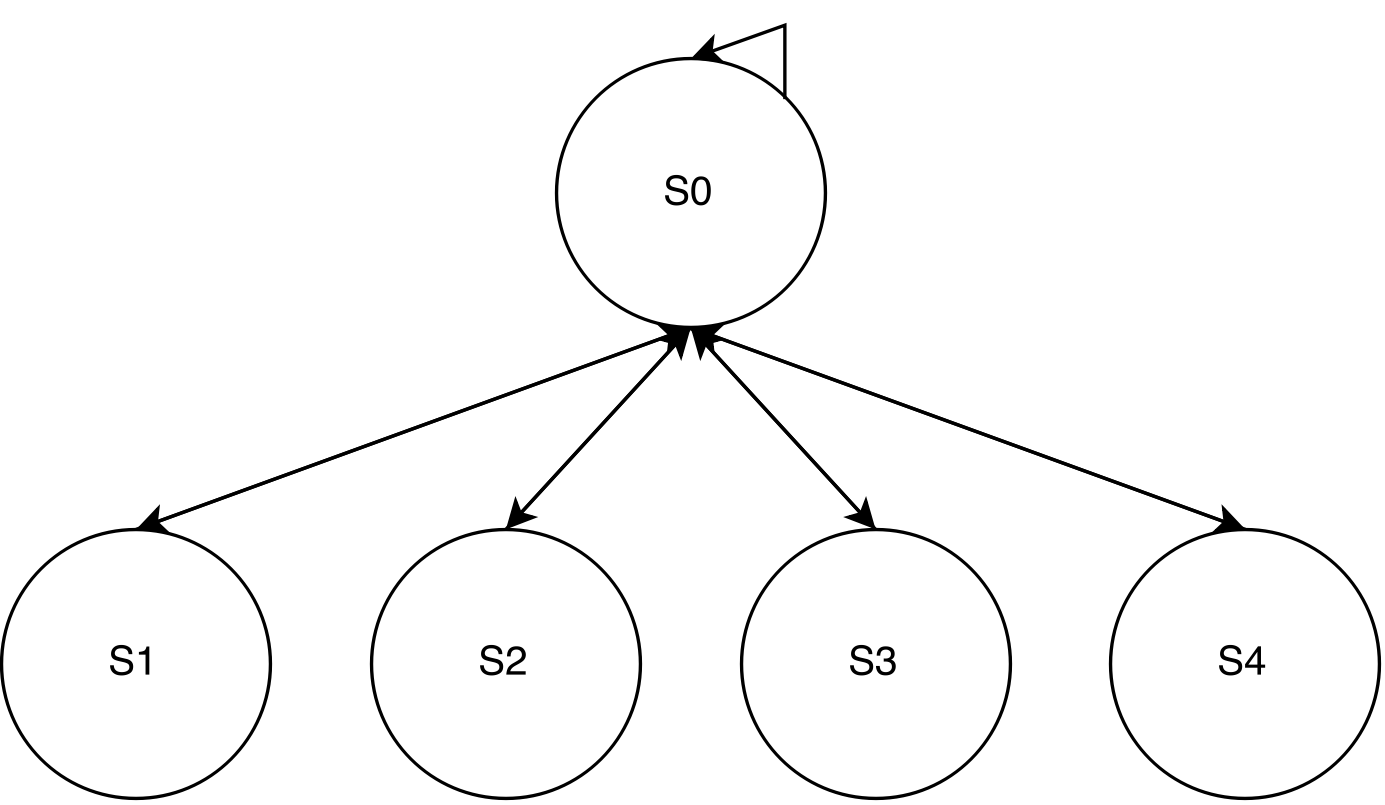
\includegraphics[width=.6\textwidth]{StatesEntity}
	\caption{Machine d'état d'une entité}
	\label{fig:StatesEntity}
	\end{center}
\end{figure}

\subsubsection{Le déplacement d'une entité}
Il est aussi important mettre en place un mécanisme de déplacement de l'entité (voir section \ref{subsubsec:deplacement}) et avec ça une direction au quelle l'unité fait face. Cette direction doit être mise-à-jour à chaque déplacement. La direction sert de référence pour tirer des projectile dans le bon endroit.

\subsubsection{Les limites de collisions}
Les limites ou \textit{Bounds} sert de zone de collision. Tous autre objets du jeu possédant la propriété \textit{IsWalkable} (voir section \ref{subsec:classdebase}) à false, se trouvera bloqué par celui-ci. De même que tout projectile ou attaque fait dans la zone engendrera des dégâts à l'entité.

\subsubsection{La portée d'action}
Une entité doit pouvoir interagir avec les autres, c'est pourquoi il faut aussi ajouter des limites d'attaques ou \textit{attack bounds}. Ce qui permet de connaître la portée des attaques de cette entité. Lorsque qu'une autre entité se trouve dans cette zone celui-ci peut se faire attaquer. Par exemple, lorsque qu'une portée d'une entité touche les limites (correspondant à la texture) d'une autre entité, celui-ci peut désormais l'attaquer (Voir figure \ref{fig:hitbox}).

\begin{figure}[h]
	\begin{center}
	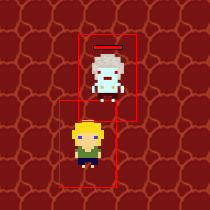
\includegraphics[width=.5\textwidth]{hitbox}
	\caption{Portée des entités}
	\label{fig:hitbox}
	\end{center}
\end{figure}

\subsubsection{La texture}
Les textures sont simple d'intégration puisqu'il fait partie de fonctionnalités que monogame offre. Il faut alors chargée une \textit{Texture2D} et le dessiner. Les animations ne sont pas fait parce que ce n'est pas une priorité.
\begin{lstlisting}[caption=Affichage de la texture sur l'écran, label=lst:afftextuecran]
Vector2 position = ScreenManager.Instance.GetCorrectScreenPosition(boundsPosA, PlayScreen.Instance.Camera.Position);
spriteBatch.Draw(this.Texture, position, Color.White);
\end{lstlisting}

\subsubsection{Le temps de dernière attaque}
Il est important de garder en mémoire le temps de la dernière attaque d'une entité, c'est ce qui permet de régler le temps qu'il y a entre chaque attaque avec les caractéristiques de celui-ci. Pour connaître le nombre d'attaque par seconde ($v$), il fait diviser $1$ par la vitesse d'attaque de l'entité ($a$). $(v = \frac{1}{a})$. Si le temps entre la dernière attaque et le temps actuel est plus grand ou égal à $v$ ($t_1 - t_2 >= v$), l'entité est libre d'effectuer une action.

\subsubsection{La mort de l'entité}
Si l'entité se retrouve avec 0 dans ses points de vie, celui-ci est mort. Une fois cette propriété à \textit{true}, l'unité se fait effacer par le gestionnaire de partie.

\subsection{Personnage jouable}
Le personnage jouable est une entité qui est contrôlée par l'utilisateur. Il possède donc des méthodes et propriétés qui lui sont propres. Le personnage a en plus :
\begin{itemize}
	\item Des sorts
	\item Des objets (\textit{items})
	\item Des actions par périphériques d'entrée
\end{itemize}
\begin{figure}[h]
	\begin{center}
	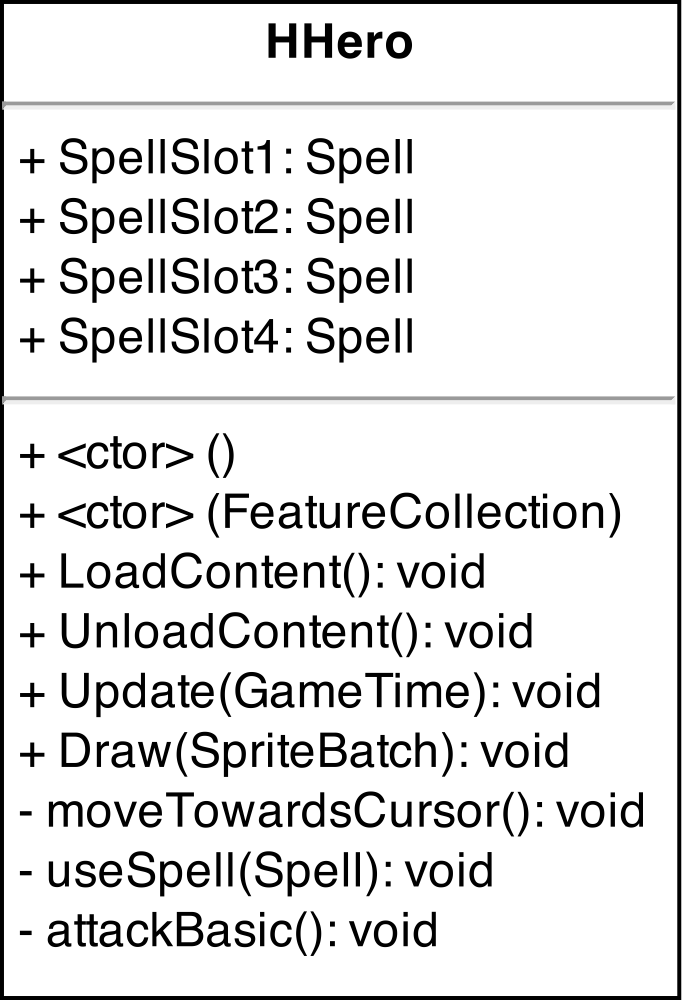
\includegraphics[width=.35\textwidth]{HHero}
	\caption{Diagramme de classe du personnage jouable}
	\label{fig:HHero}
	\end{center}
\end{figure}
\subsection{Déplacement}
\label{subsubsec:deplacement}
Le déplacement d'une entité se fait avec des vecteurs. La méthode prend deux vecteurs : la position et le point de déplacement. 
$$\vec{v} = \vec{v_1} - \vec{v_2}$$
Il faut ensuite normaliser ce vecteur qui est la direction. $|\vec{v}|$. Pour connaître la nouvelle position selon le temps et vitesse de déplacement cette formule est appliquée:
$$\vec{v} * \Delta t * s$$
$\vec{v}$ : Vecteur de direction normalisé\\
$\Delta t$ : Temps écoulé depuis le dernier \textit{Update}\\
$s$ : Vitesse de déplacement de l'entité

Il faut ensuite addition ce vecteur à la position actuel du personnage.

\subsubsection{Gestion des obstacles}
Lors d'un déplacement il est important de prendre en compte les obstacles autour de l'entité, c'est pourquoi il faut faire un vérification de la nouvelle position avec les éléments du jeu, cellule de la carte et autres entités. Si celui-ci est obstrué, on retire un des axes du vecteur de déplacement et réessaye, si il est de-nouveau obstrué, il faut remettre l'axe retiré et essayer avec l'autre. Si il n'y a toujours pas de solution, il ne faut pas validé le déplacement (voir figure \ref{fig:ObstacleManagement}).
\begin{figure}[htp]
	\begin{center}
	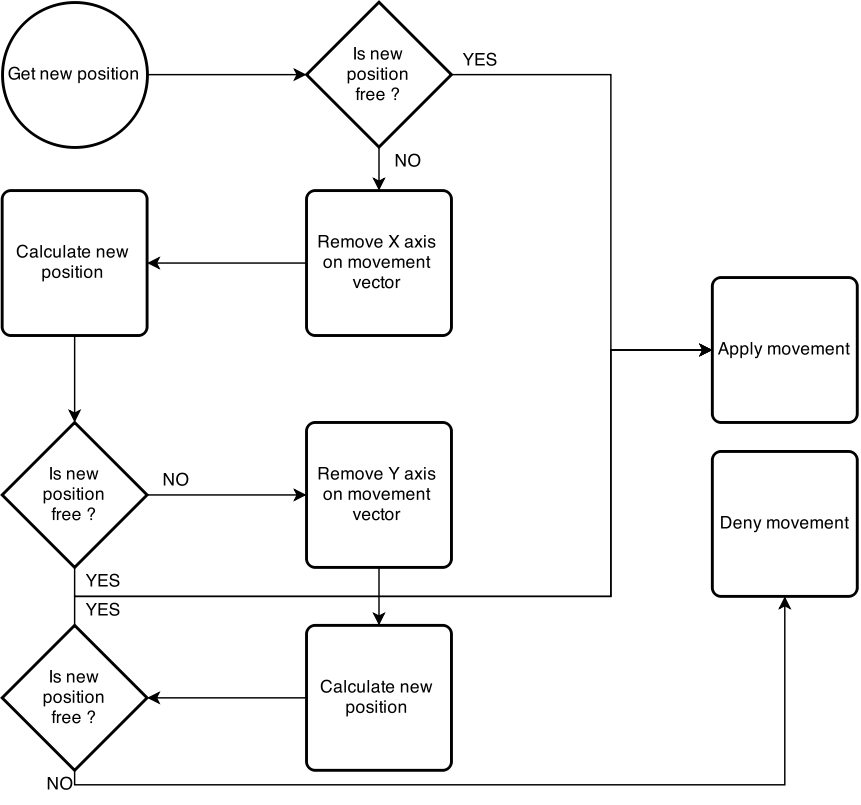
\includegraphics[width=.75\textwidth]{ObstacleManagement}
	\caption{Diagramme de flux du management d'obstacle}
	\label{fig:ObstacleManagement}
	\end{center}
\end{figure}

\subsection{Ennemis}
Les ennemis sont des entité possédant une "intelligence" contrôlée par l'ordinateur. Cette unité possède plus de zone de détection pour faire illusion d'une intelligence pour que le jeu soit plus jouable. Les propriétés ajouté sont :
\begin{description}[labelindent=0.5cm]
	\item[FieldOfView] La zone de détection
	\item[IsAlerted] L'ennemi à détecter le joueur
\end{description}

Pour que cet entité détecte des joueur, une zone de détection. Cette zone de détection est faite avec un FRectangle (voir section \ref{subsec:intersections}) qui permet de voir si les limites du joueur et de l'ennemi se touchent. Une fois détecter cette zone agrandi et l'entité passe en mode alerte jusqu'à qu'il perde de vue le joueur (voir figure \ref{fig:DetectionJoueur}).

\begin{figure}[htp]
	\begin{center}
	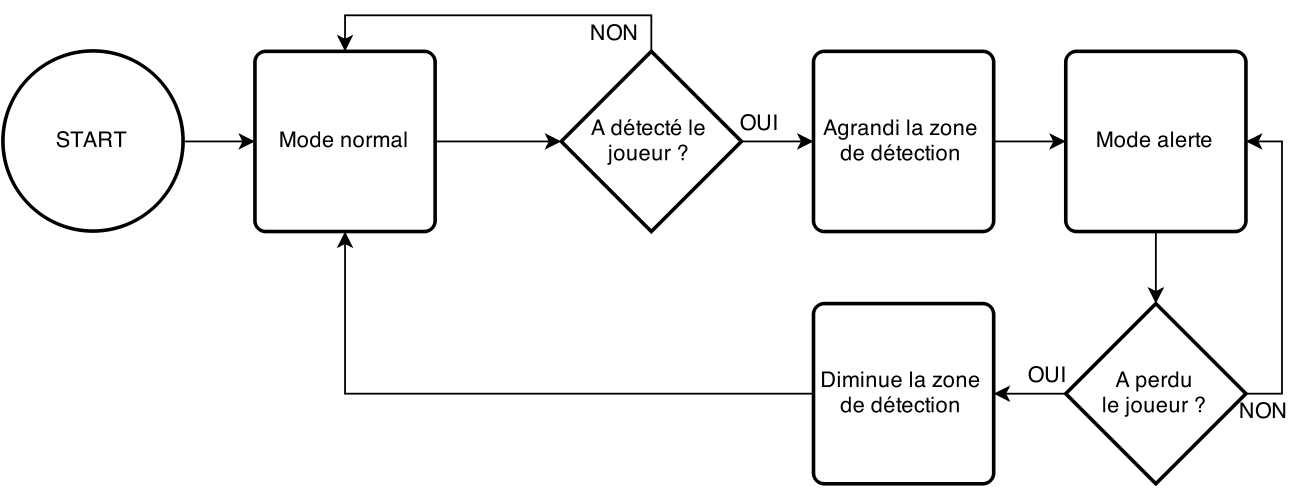
\includegraphics[width=.8\textwidth]{DetectionJoueur}
	\caption{Diagramme de flux de la détection des hostiles}
	\label{fig:DetectionJoueur}
	\end{center}
\end{figure}

\subsection{Objets - \textit{items}}
Les \textit{items} sont des objets que le personnage jouable peut ramasser et stocker dans son inventaire. Il peut de même les équiper sur soit. Les items possèdent des caractéristiques (voir section \ref{subsec:caracteristiques}), une fois que le personnage joueur équipe un item, il ajoute les caractéristiques de l'item sur soit grâce au manager de caractéristiques (voir listing \ref{lst:maxforceentity} pour un exemple de calcul du manager).
\begin{figure}[h]
	\begin{center}
	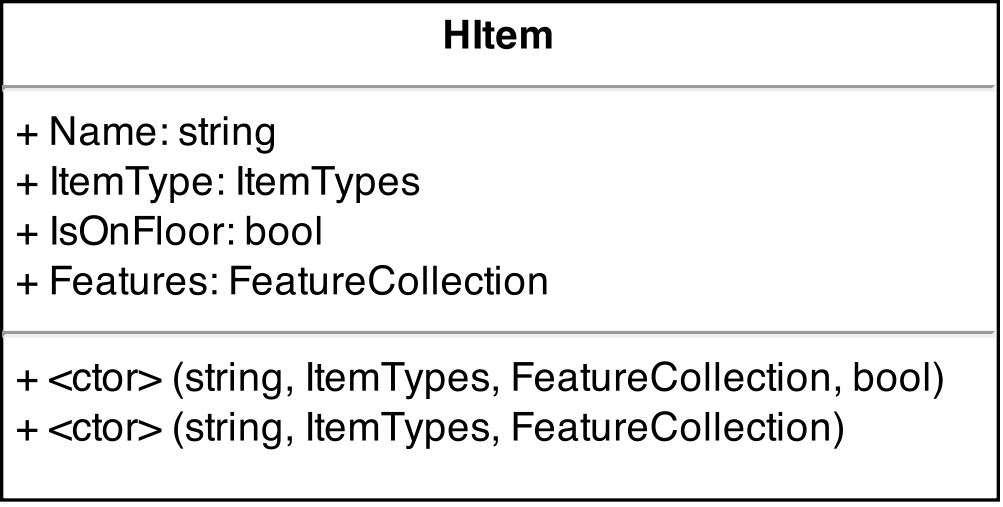
\includegraphics[width=.4\textwidth]{HItem}
	\caption{Diagramme de classe de HItem}
	\label{fig:HItem}
	\end{center}
\end{figure}
\subsection{Attaques}
\subsubsection{Corps-à-corps}
Les attaque corps à corps peuvent seulement toucher une autre entité. La cible choisi doit se trouver dans la zone d'attaque au corps-à-corps. Lui infligeant ainsi des dégâts selon les caractéristiques. Voir listing \ref{lst:basicmeleeattack}.
\begin{lstlisting}[caption=Attaque au corps-à-corps, label=lst:basicmeleeattack]
/// <summary>
/// Basic melee attack
/// </summary>
/// <param name="target">Targeted enemy</param>
public void BasicMeleeAttack(HEntity target, GameTime gameTime)
{
	// Gets the current time of the game
	double currentTime = gameTime.TotalGameTime.TotalSeconds;
	// Calculates the number of seconds per attack
	float secPerAttack = 1f / this.ActualFeatures.AttackSpeed;
	
	// If the attack can be made
	if (currentTime - this._lastAttackTime >= secPerAttack)
	{
		float minDmg = this.ActualFeatures.MinimumDamage;
		float maxDmg = this.ActualFeatures.MaximumDamage;
		float receivedDamage = (float)this._rand.NextDouble();
		receivedDamage = (maxDmg - minDmg) * receivedDamage + minDmg;
		float realReceivedDamage = this.FeatureCalculator.GetReceivedPhysicalDamage(receivedDamage);
		realReceivedDamage = realReceivedDamage * (this.ActualFeatures.Strenght / 100 + 1);
		target.ActualFeatures.LifePoints -= realReceivedDamage;
		this._lastAttackTime = currentTime;
	}
}
\end{lstlisting}
\subsubsection{Distance}
Les attaque à distance peuvent seulement toucher une autre entité avec le projectile. Le projectile ne peut pas aller plus loin que le zone d'attaque à distance et peut seulement toucher une entité, lui infligeant ainsi des dégâts selon les caractéristiques.
\subsection{Sorts}
\section{Outils de développement}
\subsection{Primitives 2D}
Malheureusement, Monogame n'offre pas de primitives 2D pour dessiner sur l'écran, c'est-à-dire les points, les ligne, les rectangles, les polygones et les ellipses. C'est pourquoi il est nécessaire de faire une classe primitive 2D (voir figure \ref{fig:Primitives2D}).
\begin{figure}[h]
	\begin{center}
	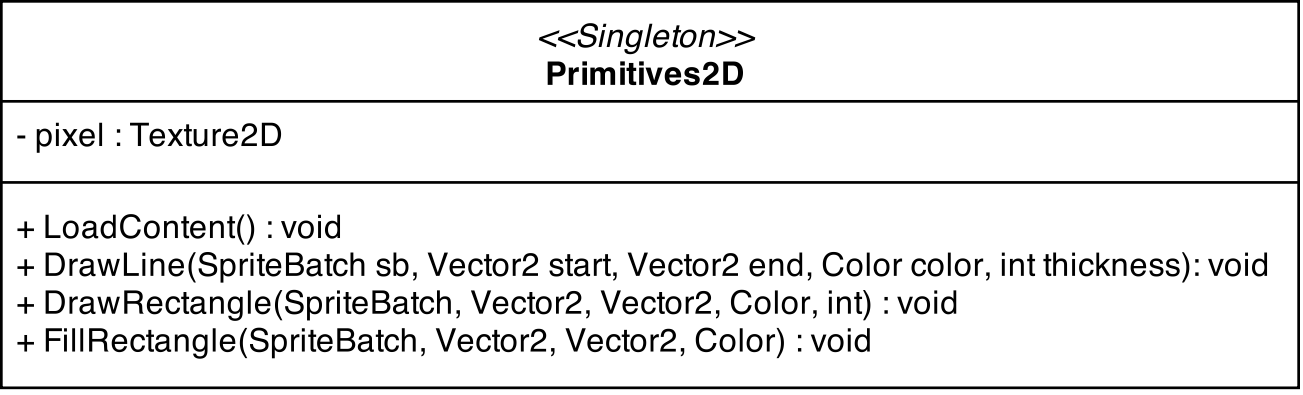
\includegraphics[width=0.7\textwidth]{Primitives2D}
	\caption{Diagramme de classe des primitives 2D}
	\label{fig:Primitives2D}
	\end{center}
\end{figure}
\subsubsection{Les méthodes}
\paragraph{LoadContent} est ce qui permet de créer le pixel par défaut avec un teinture blanche. Ce pixel de type Texture2D est indispensable, parce que c'est celui-ci qui sera manipuler pour faire des divers formes.
\paragraph{DrawLine} dessine une line entre deux points spécifiés.
\paragraph{DrawRectangle} dessine un rectangle entre deux points spécifiés.
\paragraph{FillRectangle} dessine un rectangle plein entre deux points spécifiés.
\subsection{Intersections}
Les intersections sont la base des interactions entre les éléments du jeu. C'est pourquoi chaque entité et cellule du jeu posséde des limites. Monogame n'offre qu'une classe Rectangle avec des entiers, mais pour plus de précision il faut des nombres à virgule. C'est pourquoi la classe FRectangle (voir figure \ref{fig:FRectangle}) est faite. Il possède aussi une méthode d'intersection qui détecte si le rectangle même croise un autre.
\begin{figure}[h]
	\begin{center}
	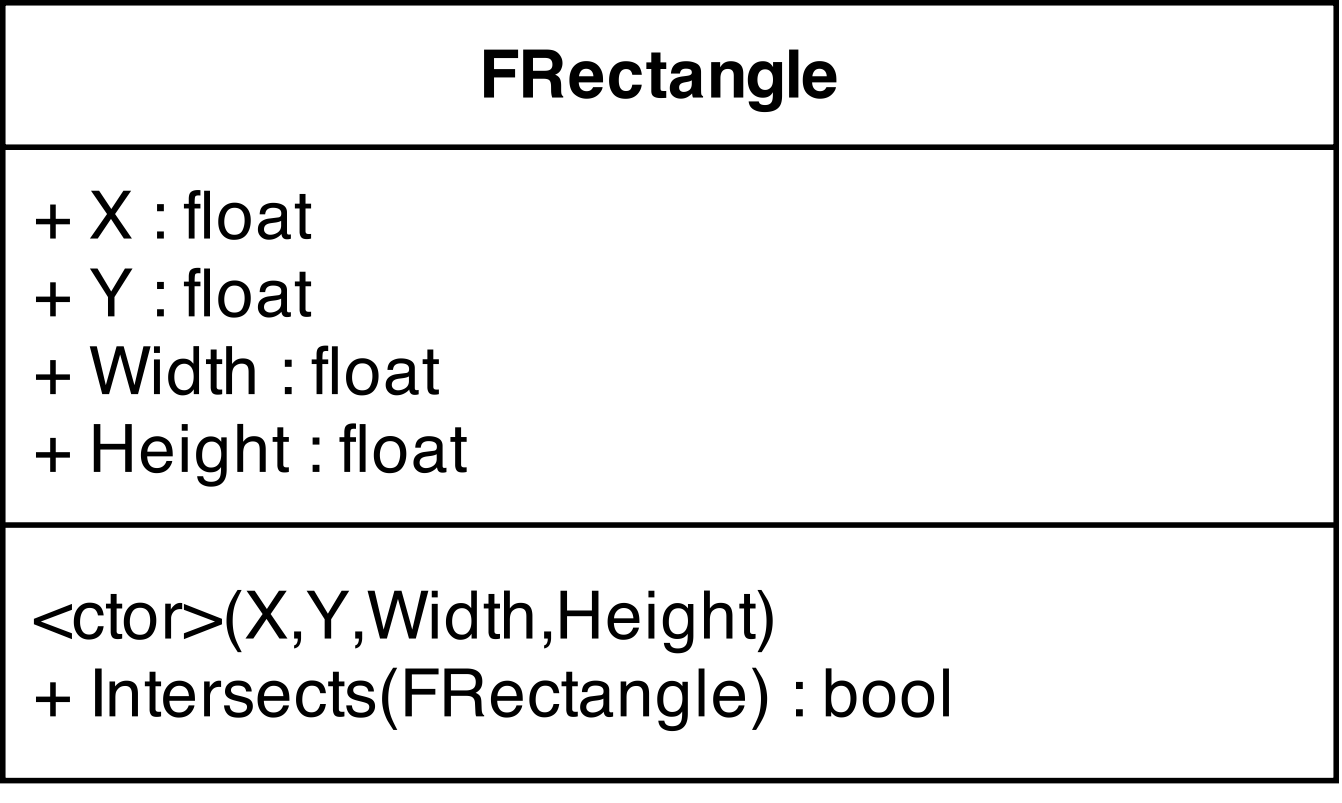
\includegraphics[width=0.7\textwidth]{FRectangle}
	\caption{Diagramme de classe de FRectangle}
	\label{fig:FRectangle}
	\end{center}
\end{figure}
\label{subsec:intersections}
\subsection{Gestion des entrées}
Il a fallu penser facon la plus efficace pour gérer les entrées. L'objectif est d'éviter de mettre des entrés directement dans la classe. C'est pourquoi la classe InputManager est faite.  Il permet de mettre à jour tous les entrées et de le placés dans des listes correspondant :

\begin{description}[labelindent=0.5cm]
	\item[DownKeys] Les touches qui viennent d'être appuyées.
	\item[PressedKeys] Les touches qui sont appuyées.
	\item[ReleasedKeys] Les touches qui viennent d'être relachées.
\end{description}

\begin{figure}[h]
	\begin{center}
	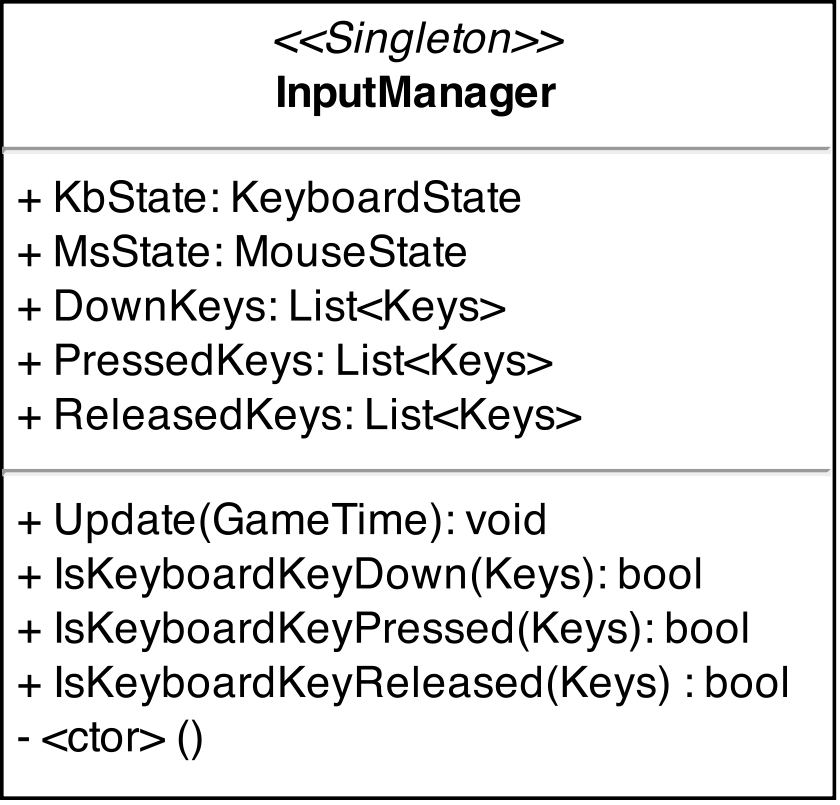
\includegraphics[width=0.35\textwidth]{InputManager}
	\caption{Diagramme de classe du manager d'entrées}
	\label{fig:InputManager}
	\end{center}
\end{figure}

Les touches ne peuvent pas se retrouvés dans plusieurs listes en même temps.

\begin{lstlisting}[caption=Mise-à-jour des entrées, label=lst:inputUpdate]
/// <summary>
/// Updates the states of the keyboard
/// </summary>
private void UpdateKeyboardInput()
{
	if (MainGame.Instance.IsActive)
	{
		this.KbState = Keyboard.GetState();
		
		// Verifies all the keys of the keyboard
		foreach (Keys key in Enum.GetValues(typeof(Keys)))
		{
			// If the key is not pressed and it is not in the release key list and is in one of the other two list
			// we add it to the released key list and remove it in the others
			if (this.KbState.IsKeyUp(key) && !this.IsKeyboardKeyReleased(key) &&
			(this.IsKeyboardKeyPressed(key) || this.IsKeyboardKeyDown(key)))
			{
				this.DownKeys.Remove(key);
				this.PressedKeys.Remove(key);
				this.ReleasedKeys.Add(key);
			}
			else if (this.KbState.IsKeyUp(key) && this.IsKeyboardKeyReleased(key)) // If it is already in the released key list
			{        // remove it
				this.ReleasedKeys.Remove(key);
			}
			else
			{
				// If the key is down and is not yet pressed
				if (this.KbState.IsKeyDown(key) && !this.IsKeyboardKeyDown(key) && !this.IsKeyboardKeyPressed(key))
				{
				// remove it from the other lists (to be sure)
					this.ReleasedKeys.Remove(key);
					this.PressedKeys.Remove(key);
					this.DownKeys.Add(key); // and add it to the down key list
				}
				else if (this.KbState.IsKeyDown(key) && !this.IsKeyboardKeyPressed(key)) // If it's already in the down key list
				{                                                                   // and isn't in the pressed list
					this.DownKeys.Remove(key); // remove it from the other lists
					this.ReleasedKeys.Remove(key);
					this.PressedKeys.Add(key); // add it to the pressed list
				}
			}
		}
	}
	else
	this.KbState = new KeyboardState();
}
\end{lstlisting}
\subsection{Sérialisation XML}
Il est important de pouvoir serialisé les objets en XML. Ceci permet d'ajouter du contenu facilement et sans toucher au code source. C'est pourquoi la classe XmlManager est générique. Il permet de sérialisé tous les objets si ceux-ci sont approprié pour la sérialisation (voir figure \ref{fig:XmlManager}).

\paragraph{Load} permet de charger un XML et de rendre un objet (voir listing \ref{lst:xmlload}).
\paragraph{Save} permet de sauvegarder un objet en XML.
\begin{lstlisting}[caption=Désérialisation d'un XML, label=lst:xmlload]
T instance;
using (TextReader reader = new StreamReader(path))
{
	XmlSerializer xml = new XmlSerializer(TypeClass);
	instance = (T)xml.Deserialize(reader);
}
return instance;
\end{lstlisting}
\begin{figure}[H]
	\begin{center}
	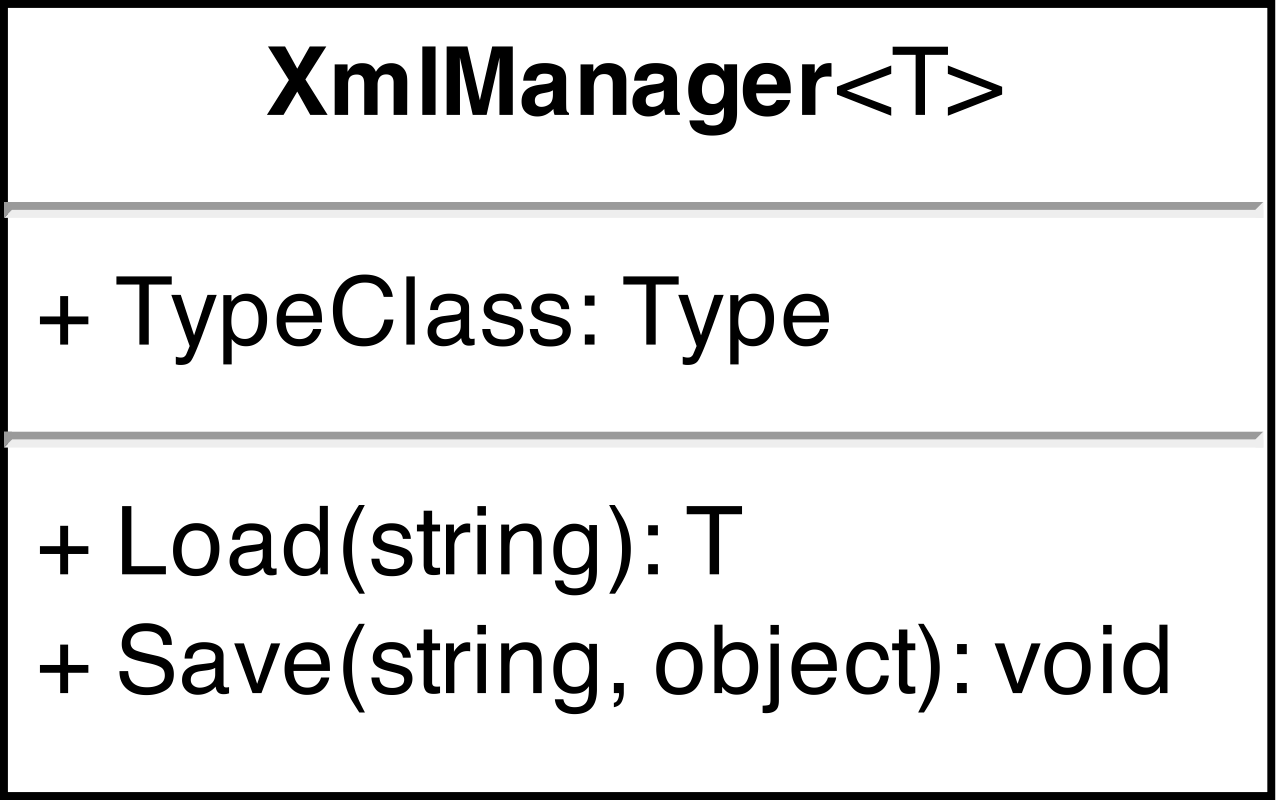
\includegraphics[width=0.35\textwidth]{XmlManager}
	\caption{Diagramme de classe du manager de sérialisation XML}
	\label{fig:XmlManager}
	\end{center}
\end{figure}

\section{Vue}
\subsection{Gestion de l'écran}
Pour centralisé les différents mode d'affichage (écran de présentation, menu et jeu), un gestionnaire d'écran qui centralise tous ces modes est nécessaire. Ce gestionnaire s'accroche sur les boucles de monogame et possède un écran actif. Cet écran actif est mise-à-jour à travers ces boucles, ce qui permet un transition fluide entre les modes. La taille d'un écran est également mémoriser dans ce gestionnaire pour garder une uniformité des écrans (voir figure \ref{screenmanagement}).
\begin{figure}[p]
	\begin{center}
	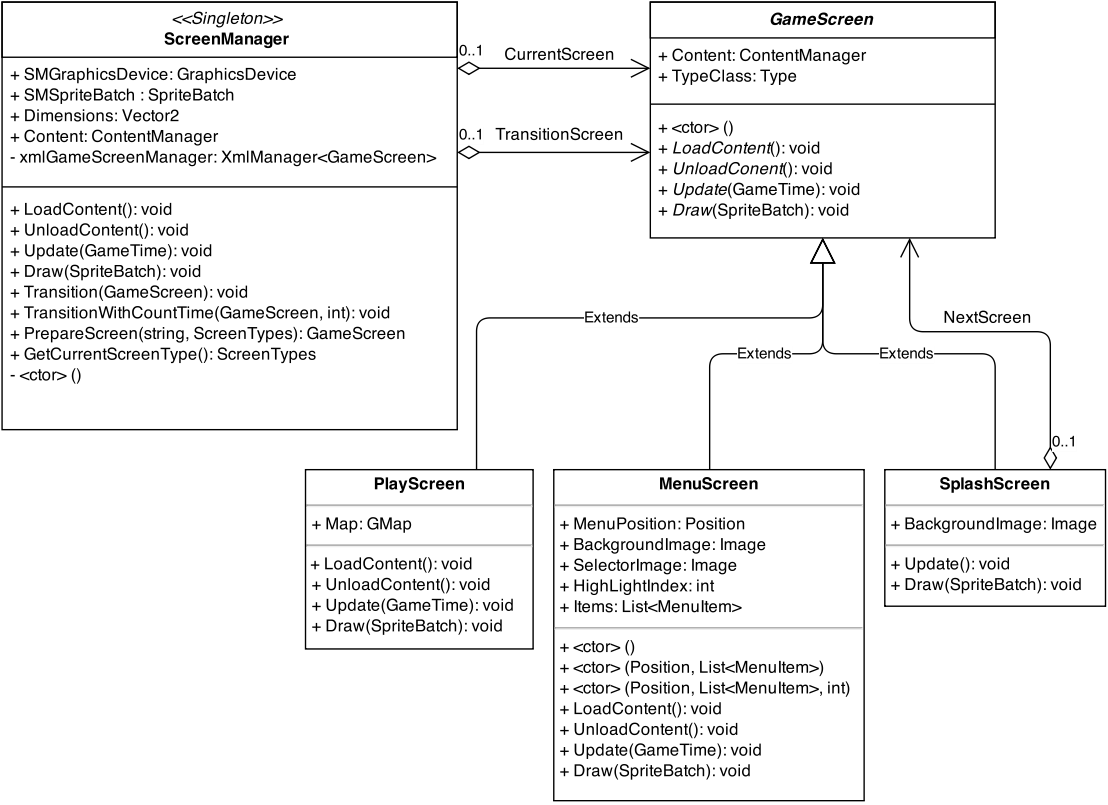
\includegraphics[width=1\textwidth]{screenmanagement}
	\caption{Diagramme de classe de la gestion d'écrans}
	\label{fig:screenmanagement}
	\end{center}
\end{figure}
\subsubsection{Les transitions}
Pour passé d'un mode d'affichage à un autre, une transition est nécessaire. C'est pourquoi la class ScreenManager contient un compteur qui garde le temps passer sur une mode d'affichage. Avec une méthode, il suffit de changé l'écran actuel après un certain temps ou lorsqu'un évennement a eu lieu. Voir le listing \ref{lst:screentransition}.
\begin{lstlisting}[caption=Transition d'écran, label=lst:screentransition]
/// <summary>
/// Transitions the screen to another one
/// </summary>
/// <param name="nextScreen"></param>
public void Transition(GameScreen nextScreen)
{
	// resets the transition variables
	this._transitionTime = 0;
	this._transitionDelayActive = false;
	this._transitionFirstCount = -1.0d;
	
	this.UnloadContent(); // unloads the content of the current screen
	this._currentScreen = nextScreen; // place the new screen
	this._currentScreen.LoadContent(); // loads the new screen
}

/// <summary>
/// Activates a screen transition for the specified time
/// </summary>
/// <param name="nextScreen">Next screen that will appear</param>
/// <param name="time">Time before transition</param>
public void Transition(GameScreen nextScreen, int time)
{
	this._transitionScreen = nextScreen;
	this._transitionTime = time;
	this._transitionDelayActive = true;
	this._transitionFirstCount = -1.0d;
}
\end{lstlisting}
\subsubsection{L'écran de base}
L'écran de base (GameScreen) est une classe absraite pour garder une même base des écrans. Un écran possède un manager de contenu qui permet la gestion, chargement et dé-chargement des contenus comme : les textures et les fonts. Une variable de type y est ajouté pour plus facilement identifier le reelle type d'écran. Bien sûr, la boucle monogame est aussi ajouté, pour offrir des possibilités de développement des écrans.
\subsubsection{L'écran de présentation}
L'écran de présentation ou \textit{SplashScreen}, est un simple écran possédant une image de fond qui porte le nom de l'auteur ainsi que son logo. Cet écran est en mode transition, cet-à-dire qu'il changera tous seul de mode ou lorsque l'utilisateur appui sur une touche.
\subsubsection{L'écran de menu}
Le menu sert d'instance d'intéraction entre le joueur et le programme. C'est pourquoi pour favoriser l'avancement du projet, il faut que le menu soit générique. C'est pourquoi son contenu s'ajoute avec des fichiers XML à l'aide du XMLManager, voir listing \ref{lst:xmlscreen}.

\begin{lstlisting}[caption=Menu en XML, label=lst:xmlscreen, language=xml]
<?xml version="1.0" encoding="utf-8" ?>
<MenuScreen>
	<Image>
	<Path>SplashScreen/main2</Path>
	<Position>
	<X>640</X>
	<Y>360</Y>
	</Position>
	</Image>
	<Items>
		<MenuItem>
		<Image>
			<Text>Play</Text>
			<Position>
				<X>100</X>
				<Y>200</Y>
			</Position>
		</Image>
		<LinkType>1</LinkType>
		<Id>1</Id>
		</MenuItem>
		<MenuItem>
		<Image>
			<Text>Options</Text>
			<Position>
				<X>100</X>
				<Y>230</Y>
			</Position>
		</Image>
		<LinkType>1</LinkType>
		<Id>2</Id>
		</MenuItem>
	</Items>
</MenuScreen>
\end{lstlisting}
\subsection{Gestion des textures}
\label{subsec:texturemanager}
Pour maintenir un jeu génerique, il faut aussi rendre le texture disponible depuis un endroit pour le centralisé. C'est pourquoi les textures sont tous chargé avec des fichiers XML au lancement du jeu. Ce qui permet un modifiction facile des textures (voir figure \ref{fig:TextureManager}). La classe charge d'abords une liste XML qui contients tous les liens des textures, ensuite il charge les textures.

\begin{center}
	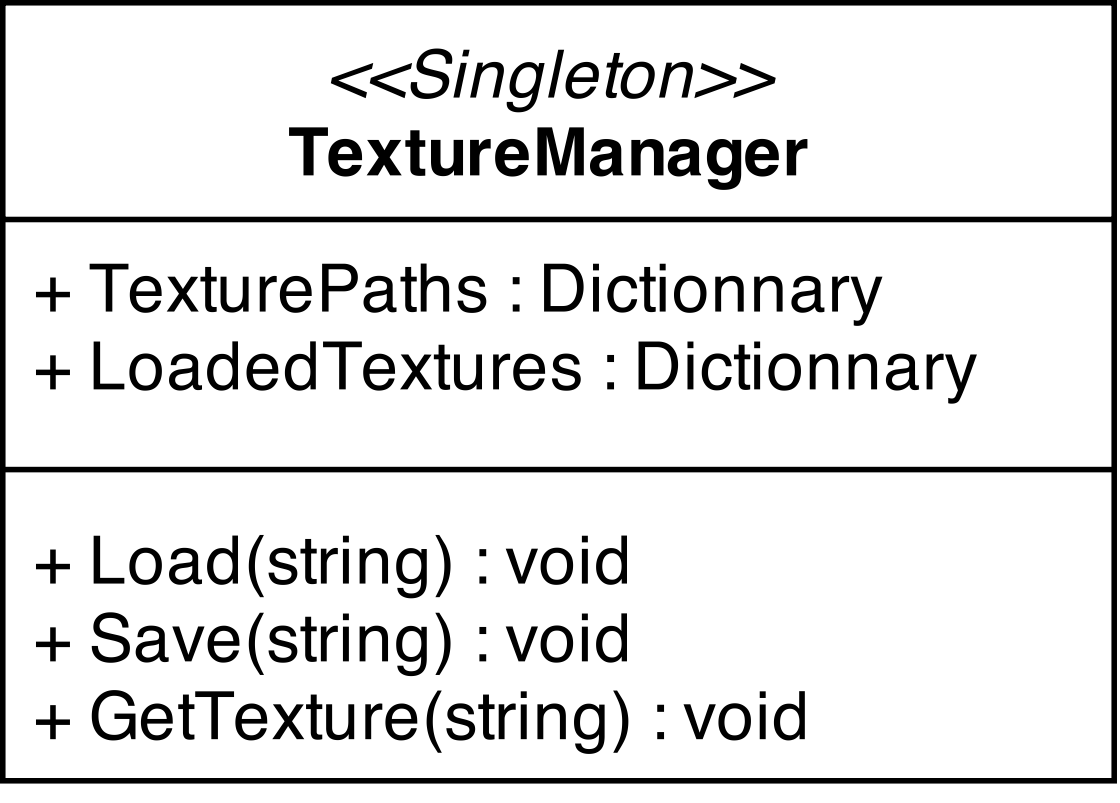
\includegraphics[width=.5\textwidth]{TextureManager}
	\caption{Diagramme de classe de la gestion de textures}
	\label{fig:TextureManager}
	\end{center}
\end{figure}
\newpage
% --------------------------------------------------
\chapter{Conclusion}

\newpage
% --------------------------------------------------
\chapter{Annexes}
\section{Planning}
Le planning du projet se décompose en plusieurs parties :\\
\begin{description}
	\item[Code backbone] Cœur du projet sur le quel le jeu se repose
	\item[Code essentiel] Éléments du jeu qui sont essentiels
	\item[Contenu] Contenu du jeu (Graphiques, Objets, etc.)
	\item[Tests] Tests pour vérifier l'intégralité du jeu
	\item[Poster] Poster préparer pour le projet
	\item[Documentation] Documentation technique du projet
\end{description}
\subsection{Initial}
% avril
\begin{figure}[H]
	\begin{center}
	\begin{ganttchart}[vgrid, hgrid, y unit title=1cm, y unit chart=0.7cm, x unit=0.8cm]{1}{14}
	    \gantttitle{Avril 2015}{14} \ganttnewline
	
	    \gantttitle{13}{1} % 1
	    \gantttitle{14}{1} % 2
	    \gantttitle{15}{1} % 3
	    \gantttitle{16}{1} % 4
	    \gantttitle{17}{1} % 5
	    \gantttitle{20}{1} % 6
	    \gantttitle{21}{1} % 7
	    \gantttitle{22}{1} % 8
	    \gantttitle{23}{1} % 9
	    \gantttitle{24}{1} % 10
	    \gantttitle{27}{1} % 11
	    \gantttitle{28}{1} % 12
	    \gantttitle{29}{1} % 13
	    \gantttitle{30}{1} \ganttnewline % 14
	    
	    \ganttbar[bar/.append style={fill=red}]{Code backbone}{6}{12} \ganttnewline
	    \ganttbar[bar/.append style={fill=red}]{Code essentiel}{12}{14} \ganttnewline
	    \ganttbar[bar/.append style={fill=blue}]{Poster}{13}{13} \ganttnewline
	    \ganttbar[bar/.append style={fill=blue}]{Documentation}{1}{14} \ganttnewline
	    \ganttmilestone{Rendu inter. doc. + poster}{14}
	\end{ganttchart}
	\caption{Planning initial du mois d'avril}
	\end{center}
\end{figure}
% mai 1
\begin{figure}[H]
	\begin{center}
	\begin{ganttchart}[vgrid, hgrid, y unit title=1cm, y unit chart=0.7cm, x unit=0.8cm]{1}{14}
	    \gantttitle{Mai 2015}{14} \ganttnewline
	
	    \gantttitle{4}{1} % 1
	    \gantttitle{5}{1} % 2
	    \gantttitle{6}{1} % 3
	    \gantttitle{7}{1} % 4
	    \gantttitle{8}{1} % 5
	    \gantttitle{11}{1} % 6
	    \gantttitle{12}{1} % 7
	    \gantttitle{13}{1} % 8
	    \gantttitle{15}{1} % 9
	    \gantttitle{18}{1} % 10
	    \gantttitle{19}{1} % 11
	    \gantttitle{20}{1} % 12
	    \gantttitle{21}{1} % 13
	    \gantttitle{22}{1} \ganttnewline % 14
	
	    \ganttbar[bar/.append style={fill=red}]{Code essentiel}{1}{8} \ganttnewline
	    \ganttbar[bar/.append style={fill=green}]{Contenu \& Équilibrage}{8}{14} \ganttnewline
	    \ganttbar[bar/.append style={fill=blue}]{Documentation}{1}{14}
	\end{ganttchart}
	\caption{Planning initial de la première partie du mois de mai}
	\end{center}
\end{figure}
% mai 2
\begin{figure}[H]
	\begin{center}
	\begin{ganttchart}[vgrid, hgrid, y unit title=1cm, y unit chart=0.7cm, x unit=0.8cm]{1}{6}
	    \gantttitle{Mai 2015}{4}
	    \gantttitle{Juin 2015}{2} \ganttnewline
	
	    \gantttitle{26}{1} % 1
	    \gantttitle{27}{1} % 2
	    \gantttitle{28}{1} % 3
	    \gantttitle{29}{1} % 4
	    \gantttitle{1}{2} \ganttnewline % 5
	
	    \ganttbar[bar/.append style={fill=green}]{Contenu \& Équilibrage}{1}{1} \ganttnewline
	    \ganttbar[bar/.append style={fill=yellow}]{Tests}{2}{4} \ganttnewline
	    \ganttbar[bar/.append style={fill=blue}]{Documentation}{1}{5} \ganttnewline
	    \ganttmilestone{Rendu final}{6}
	\end{ganttchart}
	\caption{Planning initial de la deuxième partie du mois de mai et le mois de juin}
	\end{center}
\end{figure}
\newpage
\subsection{Final}
\begin{figure}[H]
	\begin{center}
	\begin{ganttchart}[vgrid, hgrid, y unit title=1cm, y unit chart=0.7cm, x unit=0.8cm]{1}{14}
	    \gantttitle{Avril 2015}{14} \ganttnewline
	
	    \gantttitle{13}{1} % 1
	    \gantttitle{14}{1} % 2
	    \gantttitle{15}{1} % 3
	    \gantttitle{16}{1} % 4
	    \gantttitle{17}{1} % 5
	    \gantttitle{20}{1} % 6
	    \gantttitle{21}{1} % 7
	    \gantttitle{22}{1} % 8
	    \gantttitle{23}{1} % 9
	    \gantttitle{24}{1} % 10
	    \gantttitle{27}{1} % 11
	    \gantttitle{28}{1} % 12
	    \gantttitle{29}{1} % 13
	    \gantttitle{30}{1} \ganttnewline % 14
	    
	    \ganttbar[bar/.append style={fill=red}]{Code backbone}{7}{14} \ganttnewline
	    \ganttbar[bar/.append style={fill=blue}]{Poster}{11}{11}
	    \ganttbar[bar/.append style={fill=blue}]{}{13}{13}
	    \ganttnewline
	    \ganttbar[bar/.append style={fill=blue}]{Documentation}{1}{8}
	    \ganttbar[bar/.append style={fill=blue}]{}{11}{13}
	    \ganttnewline
	    \ganttmilestone{Rendu inter. doc. + poster}{14}
	\end{ganttchart}
	\caption{Planning final du mois d'avril}
	\end{center}
\end{figure}
% mai 1
\begin{figure}[H]
	\begin{center}
	\begin{ganttchart}[vgrid, hgrid, y unit title=1cm, y unit chart=0.7cm, x unit=0.8cm]{1}{14}
	    \gantttitle{Mai 2015}{14} \ganttnewline
	
	    \gantttitle{4}{1} % 1
	    \gantttitle{5}{1} % 2
	    \gantttitle{6}{1} % 3
	    \gantttitle{7}{1} % 4
	    \gantttitle{8}{1} % 5
	    \gantttitle{11}{1} % 6
	    \gantttitle{12}{1} % 7
	    \gantttitle{13}{1} % 8
	    \gantttitle{15}{1} % 9
	    \gantttitle{18}{1} % 10
	    \gantttitle{19}{1} % 11
	    \gantttitle{20}{1} % 12
	    \gantttitle{21}{1} % 13
	    \gantttitle{22}{1} \ganttnewline % 14
	
	    \ganttbar[bar/.append style={fill=red}]{Code essentiel}{1}{14} \ganttnewline
	    \ganttbar[bar/.append style={fill=green}]{Contenu \& Équilibrage}{20}{22} \ganttnewline
	    \ganttbar[bar/.append style={fill=blue}]{Documentation}{10}{14}
	\end{ganttchart}
	\caption{Planning final de la première partie du mois de mai}
	\end{center}
\end{figure}
% mai 2
\begin{figure}[H]
	\begin{center}
	\begin{ganttchart}[vgrid, hgrid, y unit title=1cm, y unit chart=0.7cm, x unit=0.8cm]{1}{6}
	    \gantttitle{Mai 2015}{4}
	    \gantttitle{Juin 2015}{2} \ganttnewline
	
	    \gantttitle{26}{1} % 1
	    \gantttitle{27}{1} % 2
	    \gantttitle{28}{1} % 3
	    \gantttitle{29}{1} % 4
	    \gantttitle{1}{2} \ganttnewline % 5
	
	    \ganttbar[bar/.append style={fill=green}]{Contenu \& Équilibrage}{4}{5} \ganttnewline
	    \ganttbar[bar/.append style={fill=yellow}]{Tests}{4}{5} \ganttnewline
	    \ganttbar[bar/.append style={fill=blue}]{Documentation}{1}{5} \ganttnewline
	    \ganttmilestone{Rendu final}{6}
	\end{ganttchart}
	\caption{Planning final de la deuxième partie du mois de mai et le mois de juin}
	\end{center}
\end{figure}
\newpage
% --------------------------------------------------
\listoffigures
\listoftables
\lstlistoflistings
\end{document}